\documentclass[manuscript,screen,review]{acmart}

\usepackage{graphicx}
\usepackage{hyperref}
\usepackage[utf8]{inputenc}
\usepackage{booktabs}
\usepackage{url}
\usepackage{comment}
\usepackage{microtype}
\usepackage{siunitx}
\usepackage{subcaption}
\sisetup{output-exponent-marker=\ensuremath{\mathrm{e}}}
\usepackage{wrapfig}
\usepackage{tabularx}
\usepackage{ragged2e}

\pdfstringdefDisableCommands{%
  \def\unskip#1{<#1>}%
}

%%
%% \BibTeX command to typeset BibTeX logo in the docs
\AtBeginDocument{%
  \providecommand\BibTeX{{%
    Bib\TeX}}}

%% Rights management information.  This information is sent to you
%% when you complete the rights form.  These commands have SAMPLE
%% values in them; it is your responsibility as an author to replace
%% the commands and values with those provided to you when you
%% complete the rights form.
% \setcopyright{acmcopyright}
% \copyrightyear{2018}
% \acmYear{2018}
% \acmDOI{XXXXXXX.XXXXXXX}

%% These commands are for a PROCEEDINGS abstract or paper.
% \acmConference[Conference acronym 'XX]{Make sure to enter the correct
%   conference title from your rights confirmation email}{June 03--05,
%   2018}{Woodstock, NY}
%%
%%  Uncomment \acmBooktitle if the title of the proceedings is different
%%  from ``Proceedings of ...''!
%%
%%\acmBooktitle{Woodstock '18: ACM Symposium on Neural Gaze Detection,
%%  June 03--05, 2018, Woodstock, NY}
% \acmPrice{15.00}
% \acmISBN{978-1-4503-XXXX-X/18/06}


%%
%% Submission ID.
%% Use this when submitting an article to a sponsored event. You'll
%% receive a unique submission ID from the organizers
%% of the event, and this ID should be used as the parameter to this command.
%%\acmSubmissionID{123-A56-BU3}

\renewcommand\UrlFont{\color{blue}\rmfamily}

%%
%% end of the preamble, start of the body of the document source.
\begin{document}

% Per ACM Computing Surveys Call:

% https://dl.acm.org/journal/csur/author-guidelines

% The ACM Computing Surveys publishes surveys of and tutorials on areas of computing research or practice.
% Long paper (ours)
%   Summarizes and organizes recent research results in a novel way 
%   Integrates and adds understanding to work in the field
%   Assumes a general knowledge of the area
%   Emphasizes 
%     Classification of the existing literature
%     Developing a perspective on the area
%     Evaluating trends
% Length
%   Should normally not exceed 35 pages, including references
%   When justified, additional material may be considered or published in an electronic supplement 
%   You will need to go through the manuscript and indicate which pages will form your 35 pages for publication and which pages are for the electronic supplement
%   Manuscripts of excessive length may be rejected without review
% Use of the ACM Journals/Transactions LaTeX style is encouraged to ensure proper formatting
% A footnote on the first page should acknowledge funding sources and presentations
% Author's current address should be given in a footnote on the first page.
% 


%%
%% The "title" command has an optional parameter,
%% allowing the author to define a "short title" to be used in page headers.
\title{Examining Multimodal Methods for Analyzing Learning and Training Environments: A Systematic Literature Review}

%%
%% The "author" command and its associated commands are used to define
%% the authors and their affiliations.
%% Of note is the shared affiliation of the first two authors, and the
%% "authornote" and "authornotemark" commands
%% used to denote shared contribution to the research.

\author{Anonymous Author 1}
\email{anonymous@anonymous.edu}
\orcid{XXXX-XXXX-XXXX}
\affiliation{%
  \institution{Anonymous University}
  \streetaddress{Address}
  \city{City}
  \state{State}
  \country{Country}
  \postcode{Postal Code}
}

\author{Anonymous Author 2}
\email{anonymous@anonymous.edu}
\orcid{XXXX-XXXX-XXXX}
\affiliation{%
  \institution{Anonymous University}
  \streetaddress{Address}
  \city{City}
  \state{State}
  \country{Country}
  \postcode{Postal Code}
}

\author{Anonymous Author 3}
\email{anonymous@anonymous.edu}
\orcid{XXXX-XXXX-XXXX}
\affiliation{%
  \institution{Anonymous University}
  \streetaddress{Address}
  \city{City}
  \state{State}
  \country{Country}
  \postcode{Postal Code}
}

\author{Anonymous Author 4}
\email{anonymous@anonymous.edu}
\orcid{XXXX-XXXX-XXXX}
\affiliation{%
  \institution{Anonymous University}
  \streetaddress{Address}
  \city{City}
  \state{State}
  \country{Country}
  \postcode{Postal Code}
}

\author{Anonymous Author 5}
\email{anonymous@anonymous.edu}
\orcid{XXXX-XXXX-XXXX}
\affiliation{%
  \institution{Anonymous University}
  \streetaddress{Address}
  \city{City}
  \state{State}
  \country{Country}
  \postcode{Postal Code}
}

\author{Anonymous Author 6}
\email{anonymous@anonymous.edu}
\orcid{XXXX-XXXX-XXXX}
\affiliation{%
  \institution{Anonymous University}
  \streetaddress{Address}
  \city{City}
  \state{State}
  \country{Country}
  \postcode{Postal Code}
}

\author{Anonymous Author 7}
\email{anonymous@anonymous.edu}
\orcid{XXXX-XXXX-XXXX}
\affiliation{%
  \institution{Anonymous University}
  \streetaddress{Address}
  \city{City}
  \state{State}
  \country{Country}
  \postcode{Postal Code}
}

\renewcommand{\shortauthors}{Anonymous et al.}

% Per ACM: 
%   Abstract should be at most 100 words long and consist of short, direct sentences.
%   Should state the objectives of the work
%   Summarize the results
%   Give the principal conclusions
%   Do not use the first person
%   Do not display mathematics
%   Do not use citation reference numbers
%   Try to avoid starting with the words "This paper ..."


% Discuss the need for mid-fusion versus early fusion
\begin{abstract}
    
\end{abstract}

%%
%% The code below is generated by the tool at http://dl.acm.org/ccs.cfm.
%% Please copy and paste the code instead of the example below.
%%

% Per ACM:

% Content Indicators

% Three types of content indicators must be assigned: (1) general terms, (2) subject descriptors, and (3) keywords and phrases. The first two items are selected from the 2012 ACM Computing Classification Scheme. Select as many of these as may be applicable.

% The keywords and phrases are additional English language words that indicate the content of the submission. They should not be synonymous with those already in the classification system: they can be more specific than the subject descriptors, or they may not be covered by the existing system at all. The following guidelines may be helpful.

%     Use important terms from the title; include their synonyms, related words and words of higher or lower generic rank.
%     Use English nouns, or noun-noun and noun-adjective combinations; do not use hyphens unless the hyphenated parts are always treated as a single unit.
%     Use specific terms whose meanings are generally accepted; do not use broad catchall terms (such as "computer", "automatic", "machine", "system", "discussion", "description"); do not use private terms or acronyms that may not be generally known.
%     Do not use negative terms stressing what your paper does not do.

% \begin{CCSXML}
% <ccs2012>
%  <concept>
%   <concept_id>10010520.10010553.10010562</concept_id>
%   <concept_desc>Computer systems organization~Embedded systems</concept_desc>
%   <concept_significance>500</concept_significance>
%  </concept>
%  <concept>
%   <concept_id>10010520.10010575.10010755</concept_id>
%   <concept_desc>Computer systems organization~Redundancy</concept_desc>
%   <concept_significance>300</concept_significance>
%  </concept>
%  <concept>
%   <concept_id>10010520.10010553.10010554</concept_id>
%   <concept_desc>Computer systems organization~Robotics</concept_desc>
%   <concept_significance>100</concept_significance>
%  </concept>
%  <concept>
%   <concept_id>10003033.10003083.10003095</concept_id>
%   <concept_desc>Networks~Network reliability</concept_desc>
%   <concept_significance>100</concept_significance>
%  </concept>
% </ccs2012>
% \end{CCSXML}

% \ccsdesc[500]{Computer systems organization~Embedded systems}
% \ccsdesc[300]{Computer systems organization~Redundancy}
% \ccsdesc{Computer systems organization~Robotics}
% \ccsdesc[100]{Networks~Network reliability}

% %
% % Keywords. The author(s) should pick words that accurately describe
% % the work being presented. Separate the keywords with commas.
\keywords{multimodal data, learning environments, training environments}

\received{00 Month 2023}
% \received[revised]{12 March 2009}
% \received[accepted]{5 June 2009}

%%
%% This command processes the author and affiliation and title
%% information and builds the first part of the formatted document.
\maketitle

\section{Introduction} \label{sec:intro}

% Architecture diagram and explanation
% Caleb: May be good to use an existing architecture from one of the big names in the field. For example, this paper from Ochoa has some nice figures that we can adapt: https://solaresearch.org/wp-content/uploads/hla22/HLA22_Chapter_6_Ochoa.pdf
% Caleb: This paper also has some good figures: https://wires.onlinelibrary.wiley.com/doi/full/10.1002/widm.1458
% Caleb: https://www.sciencedirect.com/science/article/pii/S0268401218312751
% Eduardo: https://docs.google.com/presentation/d/1RuZXndKMRlnM9J_GVaoR7EK_3JrRtXZi/edit#slide=id.p3

% Introduction to LA and MMLA and its impact on everyday lives (why should we care)
%   LA: Empowering educators and assisting students in real-world situations
%       Discuss how LA mostly focused on collecting logs and video data
%   MMLA: confronting the reality that insightful data is mostly not the easy-to-collect data
%       Applied from classrooms to workplace training
%       More holistic understanding of learning and its effect on feedback
With the rapid evolution of the educational landscape, the integration of technology has revolutionized the traditional pedagogical approaches, introducing exciting possibilities of more personalized, interactive, and engaging learning experiences. Our capability of capturing larger and larger volumes of data has hardness the power to delve deeper into the dynamics of learning processes. More formally, learning analytics (LA) is at this intersection of educational and data-driven insights \cite{}. By leveraging the vast digital footprint generated by students, LA empowers educators and students alike with the ability to make informed decisions and assessments of learning. Traditionally, LA has focused on collecting and analyzing trace logs and video recordings to make inferences on student's engagement, decision making, and other pedagogical--relevant behaviors. Through these analytics, educators can better tailor their teaching strategies to enhance student's learning journey. Fundamentally, LA transforms educational practice into a dynamic and response ecosystem, where data aids our understanding of student's progress.

Multimodal learning analytics (MMLA) is born from the realization that LA's sole reliance on trace logs and video is insufficient at explaining student's behaviors \cite{}. Some of the most insightful data lies beyond the easily collectible. MMLA is founded on the principle that human communication is multifaceted, i.e. it includes a collection of other modalities like speech, body language, and physiological responses. This recognition paves the way to a more holistic understanding of education processes not only in classrooms but also in workplaces and job training settings. Via MMLA, decoding the interplay between modalities can shed light on the complexities of collaboration and social learning \cite{}.

% Research gap, motivation for the survey
%   Remark other existing multimodal and educational surveys
%   Outline how applied and scalable MMLA survey is a gap and why the gap is important to be addressed
%   Growth of MMLA in AI & ED research field
As MMLA continues to evolve and become a main staple in educational research, comprehensive literature surveys are needed for the community have consensus on its progress, short--comings, gaps, and future directions. These surveys provide valuable insights in the growth and current state of MMLA. However, a noteworthy gap exists when it comes to applied MMLA and diving deeper in how practitioners are facing implementation, feasibility, and scalability challenges. The significance of addressing this gap becomes more evident when considering the increasing use of AI in educational research. As AI technologies shape our understanding and enhancement of learning, applied MMLA research stands at the intersection of these transformative trends.

% Vision
%   State the goal of performing a methodical and diligent survey, focused on applied scalable MMLA
%   Discuss an overview of the approach taken 
%       Google Scholar API requests
%       Quantitative graph pruning
%       Methodical qualitative pruning
%       Qualitative analysis
The vision of this survey is to perform a systematic and methodical literature view approach, specifically focused on applied and scalable MMLA. As a high overview, we used SerpAPI's infrastructure to make API requests to Google Scholar search engine to automate our initial paper collection and construct a citation graph. Quantitative and qualitative pruning techniques were then employed to extract the final corpus. Through full-paper reads, the final corpus was manually catalog and annotated. The paper's meta data was then used to perform descriptive analysis of the applied MMLA literature to gain valuable insights regarding research communities, trends, limitations, and research gaps. 

% Scope
%   Mention limitation of papers possibly not being included if they don't explicitly mention the word multimodal, but justify with reference to 2013 Ochoa paper (ochoa2022multimodal said "the term Multimodal Learning Analytics was for-mally coined in 2013")
%   Mention that MMLA is prevalent in collaborative learning, but that we did not include that specific search term because we want a representative sample of the entire MMLA field as a whole with respect to learning and training enironments.
%   Add reason for no VR: Cite work regarding scalability and adoption in classrooms, video not having semantic meaning with regard to the environment.
The scope of this review extends to any publication leveraging multimodal techniques to learning and training environments by both collecting and analyzing data across multiple modalities. This includes environments that exist fully in reality (e.g. physical therapy), mixed-reality environments (e.g. manikin-based nursing training in simulated emergency rooms), and online learning environments (e.g. students learning physics via computer software). Importantly, this review does not include "virtual reality" (VR) environments due to difficulties scaling this technology in classroom settings \cite{} and video data lacking semantic meaning with respect to its environment.

% Contributions
%   Comprehensive review of the research methods applied to multimodal learning and training environments
%   Analysis of the current body of literature and future research directions
%   Congruent taxonomy and framework
%   Novel Citation graph method for corpus reduction
%   Categorization and description of MMLA literature via citation communities
The novel contributions of this work, to the best of our knowledge, are the following: 
\begin{itemize}
    \item \textbf{Comprehensive review} of the research methods applied to multimodal environments
    \item \textbf{Congruent taxonomy and framework} that reflects recent advancements in MMLA methodology
    \item \textbf{Corpus reduction} via citation graph and graph-based algorithms
    \item \textbf{Categorization and description of research communities} via community-finding Louvain graph algorithm 
\end{itemize}

% Closing for the introduction


\section{Background} \label{sec:background}

% Discuss recent, past, and prominent works
\subsection{A Brief History}

Modern research in education and the learning sciences has seen a large push toward personalizing curriculum and the educational process to individual learner needs. Throughout this transformation, many methods of learner personalization and adaptation have been developed; however, among these, data-driven methods have emerged as an extremely promising approach. This research on data-driven learner personalization has come to be known as the field of learning analytics\footnote{\href{https://www.solaresearch.org/about/what-is-learning-analytics/}{https://www.solaresearch.org/about/what-is-learning-analytics/}}. Learning analytics research focuses on the collection and analysis of learner data in order to generate insights about learner behaviors \cite{maseleno2018demystifying, Zilvinskis2017}. These insights can then drive a variety of classroom tools and interventions such as computer-based learning and intelligent tutoring environments (e.g., \cite{heffernan2014assistments, leelawong2008designing}), adaptive scaffolding (e.g., \cite{Emerson2020, basu2017learner}), teacher-feedback tools (e.g., \cite{rodriguez2018teacher, Hutchins2023}), and many other developments. 

However, persistent throughout research in the field of learning analytics is the question: \textit{What forms of data need to be collected to gain insights into learner behaviors and enable meaningful analysis of learning scenarios} \cite{vatral2022using, ochoa2017multimodal}? In early learning analytics research, this question was largely answered through considerations of practicality; that is, the data which was analyzed was the data which was practical to collect in the classroom. This meant that early research on learning analytics focused highly on analyzing data from computer-based learning environments, where researchers had significant control over the design of the environments and curriculum, and log data could be easily collected and interpreted. This work analyzing log data from computer-based learning environments has a long, rich history and helped to develop meany of the theories and methods still used in learning analytics today. Log data from computer-based environments paints a very reasonable picture of learners actions and interactions in the context of the tasks they are performing in the environment that can be used to generate a wide variety of new insights into learners \cite{hoppe2017computational, ochoa2017multimodal}. 

However, as the field of the learning analytics continues to advance, the limitations of these more traditional log-based analysis approaches has been the topic of significant and increased scrutiny \cite{ochoa2017multimodal}. For example, what if the learning or training environment does not facilitate easy action logging? This is certainly the case for environments which are more physical and less virutal than traditional computer-based learning and intelligent tutoring environments, such as traditional classrooms (see Section \ref{subsec:environmentSpectrum}). Beyond this, what if the logged data fails to capture the full context of learners' actions and behaviors? For example, computer logs may not tell any information about learner affect or collaborative conversations between learners. These questions, among many others, alongside the development and proliferation of affordable sensor devices, have lead learning analytics researchers to deploy additional sensor devices in the classroom to help close the gaps introduced by analysis of log data alone. These more complex sensors and data sources have the ability to capture a much richer variety of learner behavioral data. For example, physical movement, gestures, and postures captured through video data; dialogue captured through microphones; stress levels captured through biometric sensors; eye gaze and attention captured through eye tracking devices; etc \cite{vatral2022using}. 

By combining together all of these additional sensor devices, researchers can capture a much richer picture of learners' affective, cognitive, psychomotor, and metacognitive states and lead to more comprehensive analysis of learner behaviors \cite{blikstein2016multimodal}. This combination of multiple sensor modalities for analysis of learner behavior has come to be known as the field of multimodal learning analytics (MMLA) \cite{blikstein2013multimodal, blikstein2016multimodal, worsley_multimodal_2018}. Today, MMLA has been the subject of over a decade of concentrated research including multiple journal special issues \cite{BJETSpecialIssue}\footnote{\href{https://www.mdpi.com/journal/sensors/special_issues/multimodal_learning_analytics_sensor}{https://www.mdpi.com/journal/sensors/special\_issues/multimodal\_learning\_analytics\_sensor}}\footnote{\href{https://learning-analytics.info/index.php/JLA/announcement/view/102}{https://learning-analytics.info/index.php/JLA/announcement/view/102}}, a special interest group in the Society for Learning Analytics Research\footnote{\href{https://www.solaresearch.org/community/sigs/crossmmla-sig/}{https://www.solaresearch.org/community/sigs/crossmmla-sig/}}, an edited book \cite{MMLAHandbook}, and several systematic literature reviews \cite{Chango2022, Alwahaby2022, Shankar2018, Crescenzi2020, Mu2020, DiMitri2018, worsley_multimodal_2018}. Owing to this significant body of prior work, in this review we narrow our focus to the study of only applied research methods studies.

\subsection{Related Work} \label{subsec:related_work}

% Other literature reviews
% How are we different than others?
% Other lit reviews/surveys:
%   A review on data fusion in multimodal learning analytics and educational data mining
%   Multimodal data capabilities for learning: What can multimodal data tell us about learning?
%   Trends of Multimodal Learning Analytics: A Systematic Literature Review
Following the large wave of MMLA research, there has been various literature surveys that have provided different window views towards the MMLA landscape. For a concise list, relevant MMLA surveys include: multimodal data fusion \cite{chango_review_nodate}, conceptual model and taxonomy \cite{di_mitri_signals_2018}, statistical and qualitative assessment of literature \cite{sharma_multimodal_2020, qushem_trends_nodate}, virtual reality \cite{philippe_multimodal_2020}, technology and data engineering focused for automatic MMLA \cite{chua_technologies_2019}, and impact and ethical considerations \cite{alwahaby_evidence_2021}. Our survey fits along these by addressing the dimensions of applied and scalable MMLA. Prior surveys have touched these themes, but has not reached the level of granularity and have explore trends within applied methodologies. In the following paragraphs, we will be discussing in more detail foundational surveys that support our own framing. Our intentions are to extend/modify their existing taxonomy to more accurately reflect the current state of MMLA. 

% DI MITRI (Observability)
%   From signals to knowledge: A conceptual model for multimodal learning analytics
In \citet{di_mitri_signals_2018} survey, they proposed the Multimodal Learning Analytics Model (MLeAM), a conceptual model that describes the cyclical relationship between behavior, data, machine learning, and feedback in MMLA. Along with a comprehensive taxonomy, a key insight presented was the concept of data observability and its split of space into input and hypothesis. More precisely, \citet{di_mitri_signals_2018} states that their is an observability line acting as the boundary between these two spaces, where input space is for measurable and sensory evidence (e.g. behaviors) and the hypothesis space was reserved for human-inferred annotation (e.g. emotions, motivation, cognition, and belief). The idea of observability, which refers to the process of using AI to turn input evidence into hypotheses, has guided our understanding as we define and describe applied MMLA research in this context.

% CHANGO: (Data Fusion)
%   A review on data fusion in multimodal learning analytics and educational data mining
%   Fusion of multiple modalities and its affects in ML and EDM
%   Focus on the data fusion itself
%   Modalities mentioned: audio, video, electrodermal activity, gaze, logs, clicks, gestures, speech, writing
%   Hardware mentioned: computers, cameras, sensors, infrared imaging, eye tracking glasses
%   Used SLR template from Tranfield 2003, not Kitchenham
%   Does not have the granularity we are discussing, so currently no conflicts with our definitions
%   5 categories of data: digital, e.g. clicks and logs; physical, e.g. gestures; physiological, e.g. EEG; psychometric, e.g. mental state surveys; environmental, e.g. physical location, temperature, weather
%   Capture methods: webcam, eye trackers, electrodes, sensors, .csv files, software
%   Data collected across: data source, data type, data category, capture method
%   Fusion: early fusion (feature level, before analysis), late fusion (decision level, after analysis), hybrid
Another influential survey is \citet{chango_review_nodate}, where data fusion methodologies and practices in MMLA are its main focus. In their approach, papers were classified by data fusion technique and point, aiming to understand its impact of machine learning and educational data mining. After generating and reading their corpus, they proposed a classification scheme to determine the type of data fusion as early, late, or hybrid, depending on the stage of integration – early fusion involved concatenating features before classification, while late fusion referred to decision-level concatenation after classification. 

By combining the valuable insights from these two significant surveys, a more complete and current understanding of data fusion emerges. This improved definition seamlessly integrates the idea of observability, capturing the process of bringing together different sources of information to create a unified data representation. This definition also takes into account the distinction between measurable sensory evidence and human-inferred annotations, guided by the observability line. In the upcoming section, we further elaborate in these data fusion scheme along with refined taxonomy.

\section{Framework}
% Lens through which we are conducting this research

% Analysis RQs!

% Possible RQs:

%     1.Literature Gap In applied MMLA Methods - Answered by modalities + analysis methods bar charts
%     2.The need for mid fusion - most people are using it but no one has every classified it this way
%     3.What do communities tell us about current landscape of MMLTE?
%       -ENV GOAL/TYPE ANALYSIS VIA COMMUNITIES:
%       -Only reread 53 not 73
%       -Dives deeper into communities as requested
%       -Helps explain away the methodology question of why we didn't collect this initially, but we use this as a way to better inform the communities
%       -Condisder individual community analysis across publication
%       -Most researchers only use a few 2-5 modalities, rather than many          -motivates technical challenges and ChimeraPy within each community. Differences, reasons.
%       -Literature gap in communities: is there anything specifically that there is not a community for and would be worth having a separate community for
        % -Nature of applications methods have been applied to, what has been done, i.e., analysis 
        % -Scope: publication venues of all 73 papers, and of each individual community 

% New proposed coding scheme:
% Hierarchical: Environment Type => Environment Setting => Environment Subject => Environment Features
    % Environment Type: Learning/Training
    % Environment Setting: Physical/Virtual/Blended
    % Environment Subject: Core Science (biology, physics, etc.), Applied science (clinical settings, engineering, etc.) Math, Language Arts, Psychomotor Skills 
    % Environment Features: Gamification, multi-student, didactic, computer-based, open-ended, embodied, simulation-based, mixed reality
    

% Since the term MMLA was formally coined in 2013 (Blikstein, c/o Ochoa), it has been used to inform learning and training environments.
% Research has shown multimodal data is very often more informative than any single modality.
% Several reviews have been done on MMLA, but through various lenses: data fusion (Chango, 2022); learning objectives such as behavior, engagement, and outcome (Sharma, 2020); and MMLA trends (Qushem, 2020)
% We identified the need for a review of MMLA methods applied to multimodal data in learning and training environments. I.e., how are researchers and practitioners using MMLA to inform their environments based on the data they have?
% This review is focused on applied multimodal methods used to inform learning and training environments.
% Fully virtual environments are not included due to scalability issues in classrooms and a lack of video context relative to the environment. 
% We discover, characterize, and contrast sub-communities within MMLA with the goal of understanding trends in analysis.
% This review will provide researchers with insight into how others are applying MMLA to their learning and training environments given specific combinations of data collection mediums, modalities, analysis methods, and data fusion types.

% Definitions
%% Discuss participant tasks, participant goals, and researcher goals
For the purposes of this paper, we define a \textit{modality} as a unique attribute defined by data from one of more datastreams, where each modality conveys different information, even if derived from the same data collection medium \cite{Ochoa?}. We define \textit{multimodal} as a combination of either multiple modalities or multiple datastreams (i.e., multiple data collection mediums). For instance, the same video datastream could be used for the affect and pose modalities (one-to-many), and the affect modality could be derived from separate audio and video datastreams (many-to-one). Both examples would be considered multimodal by our definition. Additionally, we use the terms ``papers" and ``works" interchangeably in this review, as we expand our definition of ``paper" to include other publications outside of conference and journal submissions (books, for example).
 
We define a \textit{learning environment} as any environment whose explicit purpose is to foster knowledge gain and retention. This can include school classrooms, tutoring centers, online learning environments like Khan Academy, etc. Learning environments are focused on helping users gain knowledge and retain information, and they are often (though not always) open-ended. We define a \textit{training environment} as any environment whose explicit purpose is to help users achieve an end goal, such as task-proficiency or a positive outcome other than learning. This is often done through practice and repetition, and can include military training, nursing training, physical training, workplace training, etc. Training environments are task-oriented and are often (though not always), constrained. 

Importantly, the question of what exactly constitutes ``multimodal" environments and analysis is debated. Some researchers argue that the term multimodal is defined by the uniqueness of a datastream (or sensor), meaning multiple modalities cannot be derived from the same datastream \cite{}. However, we consider multiple datastreams to be indicative of \textit{multimedia} and not multimodality \cite{}. Similar disagreements occur when defining what constitutes early versus late fusion and learning versus training environment. Additionally, not all multimodal learning and training environments are analyzed via multimodal methods. A \textit{multimodal composing} environment \cite{}, for example, may involve students creating works using multiple modalities (e.g., a comic book sketch with both text and images), but researchers may opt to only analyze students' discourse while in the environment (which would be unimodal analysis, and therefore outside the scope of this review). 

Consider a paper whose sole focus is multimodal composing environments that happens to perform multimodal analysis in passing. Should this paper be included in the search space, despite not having multimodal analysis as one of its foci? In this review, we argue yes, as we are interested in the different methods researchers are using to conduct multimodal analysis and are not limiting ourselves to only papers where multimodal analysis is a primary focus. Clearly, these distinctions are quite nuanced, which is why the definitions we use in this paper are not meant to be interpreted as ground truth. They were chosen, after much discussion, based on how we wanted to characterize the scope of our review.


\subsection{Environment Spectrum}\label{subsec:environmentSpectrum} % Physical <--- Mixed ----> Virtual

% No AR/VR training environments that require learner to wear glasses in this study

One important aspect when considering the literature surrounding multimodal learning analytics (MMLA) is identifying the contexts in which these techniques are used, which mostly fall under the category continuum of learning and training (see Figure \ref{fig:ltcontinuum}). The main goals of learning environments are education and knowledge gain. These venues range from conventional classrooms to online courses and self-paced learning environments. When we categorize these environments on our continuum shown in Figure \ref{fig:ltcontinuum}, we add a second dimension, between fully physical and fully virtual, to represent this wide range of learning environments. MMLA methods applied in learning environments focus on extracting insights from various modalities such as text, audio, video, and interactions to assess students' comprehension, engagement, and progress. Educators may modify instructional tactics, spot problematic students, and improve learning materials by analyzing these multimodal signals since they provide significant insights into both individual and group learning patterns.

\begin{figure}
    \centering
    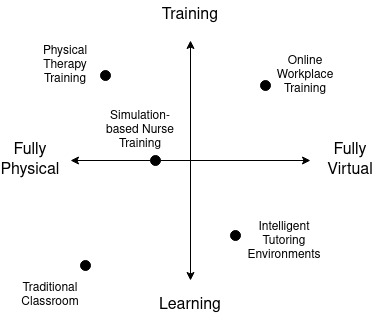
\includegraphics[width=0.5\textwidth]{img/LearningTrainingContinuum.jpg}
    \caption{Learning-Training Continuum}
    \label{fig:ltcontinuum}
\end{figure}

On the other hand, training environments are designed to improve performance and build skills. This category encompasses professional training programs, simulations, and vocational training platforms, across the same potential continuum of fully virtual to fully physical that we used to categorize learning environments. In training settings, MMLA approaches are used to evaluate data in order to track the mastery of new skills, the accomplishment of tasks, and overall performance. These insights help instructors and managers adjust training programs, spot competency gaps, and determine how prepared students are for issues in the real world. The objectives of MMLA differ in learning and training situations, calling for specific strategies that take into account the specifics of each situation, but in this paper we review literature across the spectrum of learning and training.

However, it is important to note that this division isn't always clear-cut. Some environments of study, like those populated by PhD students, blur the line between education and training. These students are learning new things in a vein similar to learning environments, but they are also increasing their research abilities and expertise, in a vein similar to a training program. Similarly, certain contexts, like game-playing platforms, defy easy classification into the learning or training categories. In these instances, MMLA methodologies must be flexibly applied, appreciating the multifaceted nature of the objectives at hand. In our categorization of all of the environments from our corpus of papers, we recognize this ambiguity in discrete categorization, but also recognize the utility of such a categorization when analyzing the research subcommunities that makeup the larger field of MMLA. As such, we perform a fuzzy qualitative discrete categorization based on discussions among the authors of where we believe each paper’s environment best fits on our continuum shown in Figure \ref{fig:ltcontinuum}.

\subsection{Data Collection Mediums} 
% Definitions
% Researcher artifacts includes field notes and also labeling of the data (i.e., manual coding). 
% Participant artifacts includes pre/post tests and the like. To qualify, all artifacts must be collected and analyzed in the pipeline and cannot be collected post hoc afterward.
% Depth camera versus regular: discuss that both are video, but depth usually used for motion modality with skeletal features
% motion capture (posyx, accelerometer, gyroscope, magnetometer)
% Make point that things like learning gains and performance can fall into multiple categories depending on where derived from, e.g., logs, surveys, student artifacts (which can also be demo information)


\subsection{Modalities} \label{sec:Modalities}
% Definitions


\subsection{Analysis Methods}
% Definitions
% Pattern extraction analysis usually refers to identifying sequences, but can be other types of patterns (include examples, revisit later). Used as catch-all for when patterns are identified but do not fall under other subsets of pattern extraction like clustering. Sequwnce mining, some HMM applications, etc.
% Define classification for our purposes as using an algorithm to predict an output in a discrete space. Mention RL paper as using RL but falling into classification category by our definition. 
% Add caveat that analysis methods refers to analysis only of the data and not of the actual analysis, unless analysis of the analysis provides more information about the data (show examples)


\subsection{Data Fusion}
% Graphic with different kinds of fusion
% Fusion definitions:
%   Early fusion. Raw, obserable data is fused directly from data collection medium and used for analysis. E.g. using raw audio signal and screen pixels, and fusing them for analysis.
%   Mid fusion. Observable features are unimodally extracted from raw data, and those extracted features are fused for analysis. E.g. extract affect from video and transcriptions from speech and fusing them for analysis. 
%   Add that we consider "cognitive load" an "observable" feature, as it comes out-of-the-box with some sensors' software (e.g. Kinect)
%   Late fusion. Unobservable features are extracted from the data, and then fused for analysis. E.g., fusing neural network output for analysis.
%   Explain: None or Other (OTH) fusion, hybrid fusion
%       cite Chango: A review on data fusion in multimodal learning analytics and educational data mining
%       "studies that do not fit into none of those three groups or in which the fusion point was not specified (Others category)"
%   Hybrid can either be separate pipelines (as traditionally defined) or multiple data types in the same pipeline

%   di mitri paper reference for observable/unobservable fusion definition: https://onlinelibrary.wiley.com/doi/full/10.1111/jcal.12288

In the realm of multimodal learning analytics (MMLA), data fusion plays a pivotal role in harnessing the power of multiple data sources to provide a more comprehensive and insightful understanding of the learning process. The process of data fusion involves combining information from various sources to create a unified dataset, thereby facilitating enhanced interpretation and analysis, when compared to analyzing only a single modality at a time. By combining data from multiple modalities, researchers and educators can uncover hidden insights into learners' cognitive states, emotions, and behaviors. This comprehensive understanding paves the way for personalized interventions and more effective pedagogical strategies. 

Within data fusion, the traditional method of categorization, as underscored by Chango et al.’s \cite{Chango2022} recent review of data fusion within MMLA, is based on three categories: early, late, and hybrid. The \textit{early fusion} approach involves combining raw data from multiple sources at the earliest stage of processing. This integration occurs before any individual modality-specific analysis, allowing for joint processing of data from different sources. By merging information early, the model can capture potential interactions and dependencies among modalities, but limited by cases where there are significant differences between data modalities and challenges surrounding the complexity and explainability of the joint modality models. The \textit{late fusion} approach involves performing separate analyses on individual modalities and then integrating their outcomes at a later stage. This method allows for specialized processing of each modality's characteristics, potentially leading to more accurate and contextually relevant insights, but limited in its ability to capture intermodal relationships that might exist. The \textit{hybrid fusion} approach aims to combine the strengths of both early and late fusion methods. In this approach, data from various sources are combined at multiple stages of processing. For instance, an initial early fusion step might be followed by separate analyses of each modality using a late fusion strategy. This allows for the exploitation of intermodal relationships while also accommodating the uniqueness of each modality's information. However, hybrid models increase the overall complexity of data analysis and require a priori decisions about which features should be combined at what points in the model pipeline. The choice of fusion method depends on several factors, including the specific problem domain, the characteristics of the available data, the desired level of interpretability, and the computational resources available.

However, we argue that this traditional three-state categorization is actually not informed enough to fully capture the complexity of multimodal analysis. After qualitative review of our paper corpus, we had significant difficulty categorizing analysis methods into just these three categories due to the ambiguity surrounding what constitutes \textit{raw features} compared to \textit{processed features}. For example, some researchers might classify the joint position data measured by a Microsoft Kinect camera as a raw feature, and thus permissible in early fusion, since it is available from the camera without any additional processing by the researchers. However, others might classify this as a processed feature, and thus a part of hybrid or late fusion, since the Kinect camera is actually computing this data from the raw depth data, regardless of whether this computation is obfuscated to the end user. Qualitatively, we noticed this pattern and disagreement among researchers with multiple modalities within our paper corpus. Motivated by this finding, we propose an additional category of data fusion, which we call \textit{mid fusion}. 

Mid-fusion represents a middle point between early fusion and late fusion, where data could be somewhat processed and transformed before being combined, but not transformed to the same extent as in late fusion. The difference here between mid and late fusion can be somewhat subtle depending on the modality, but is perhaps best explained using Di Mitri et al.’s \cite{DiMitri2018} conceptualization of the \textit{observability line}. In their work, modalities are categorized into \textit{input space}, which represents observable evidence and data that can be tracked with sensors, and \textit{hypothesis space}, which represents inferred learning labels. These two categories are separated by the \textit{observability line}, which they describe as "a line of separation between the observable evidence and all the possible interpretations" \cite{DiMitri2018}. In our new framework for categorizing data fusion, \textit{early fusion} represents combination without any initial processing, \textit{mid fusion} represents combination of features that have had prior processing that stays within the input space (i.e., still observable features), and \textit{late fusion} represents combination of features that have had prior processing that crosses the observability line into the hypothesis space (i.e., no longer directly observable).

For example, consider the same Kinect sensor discussed earlier. In this case, the raw pixel values from the camera image or the raw depth values from the depth sensor would be considered unprocessed observable features and candidates for early fusion. However, the joint position coordinates output by the camera SDK would be considered observable processed features, and thus candidates for mid fusion, since they are derived from other observable data, but still remain directly observable. Beyond this, if a researcher used the joint position data as input to another model which estimated a measure of motivation, for example, then this motivation construct would only be a candidate for late fusion, since we have now crossed the observability line. 

This classification is still somewhat qualitative and up to a researcher's interpretation. As described by Di Mitri et al., "The distinction between observable/unobservable is conceptual and can vary in practice." \cite{DiMitri2018}; however, we believe that this additional data fusion category helps to resolve some of the ambiguity related to the original categorization scheme and is useful for identifying the sub-communities of MMLA based on which methods researchers have applied. For a concrete definition of the modalities that we consider oberservable for the categorization in this paper, see section \ref{sec:Modalities}. In addition to the early, mid, late, and hybrid data fusion categories, in this paper, following the methodology of Chango et al. \cite{Chango2022}, we add an \textit{other} category to catch studies that do not fit into one of those four groups or in which the fusion point was not specified.

\subsection{Environment Goals}

\section{Methods} \label{sec:methods} % How our literature view was done

% Overview of methods section to include lit search, study selection, feature extraction, and analysis methods

\subsection{Literature Search} \label{subsec:literature_search}

This literature review examines contemporary multimodal analytics methods applied to learning and training environments. Our aim is to collect all pertinent papers published between 1/1/2017 and 10/22/2022. The proceeding paragraphs detail the methods used to construct our literature corpus and the efforts taken to consider all relevant papers, which we then distill via both quantitative (network analysis) and qualitative (quality control) methods to a manageable amount of works we believe to be representative of the current state of the field. In doing so, we introduce a novel graph-based study selection approach that uses a directed citation graph to exclude irrelevant works based on a paper's incoming and outgoing citations. To the authors' knowledge, this approach has not been previously used for distilling a literature review corpus. Our procedure for performing the quality control portion of this literature review is adapted from Barbara Kitchenham's ``Procedures for Performing Systematic Reviews" \cite{kitchenham2004procedures}.

Our literature search consisted of 42 queries agreed upon and defined by the authors as being representative of the body of works this literature review would be conducted on. Instead of performing our queries manually, our approach leverages programmatic querying via API-based web scraping for Google Scholar. There are multiple tools for scraping Google Scholar information, such as \href{https://pypi.org/project/scholarly/}{scholarly} and \href{https://github.com/venthur/gscholar}{gscholar}. Ultimately, we employed \href{https://serpapi.com/google-scholar-api}{SerpAPI}, a proprietary third-party Google Scholar web scraping API, for its most essential feature: organic web results. Other API tools' results are not organic, i.e., a query made via the API and one manually queried in a browser-based environment will produce two different sets of results.

Queries were posed via API request to Google Scholar for papers published between 1/1/2017 and 10/22/2022 (the date of the literature search). 2017 was collectively agreed upon as being the best cutoff date for inclusion in our search due to the rapid technological advancements in the field over the past 5 years. Several papers prior to 2017 are discussed in Section \ref{sec:background}, as they are seminal works; however, they are not considered for inclusion in our corpus. 

For the literature search, this review's authors decided on 14 distinct search strings, and each string was searched 3 times with a different spelling of the word \textit{multimodal} --- multimodal, multi-modal, and multi modal --- prepended to it. The 14 search strings are enumerated in Table \ref{tab:search_terms}.\footnote{The term ``xai" was originally included in the search queries due to the authors' interest in exploring explainable AI methods applied to learning and training environments. Unfortunately, the field is still nascent, and no usable query results were returned given our search criteria.}

\begin{table}[htbp]
    \renewcommand{\arraystretch}{1.3}%
    \centering
    \caption{Search strings used for the literature search.}
    \begin{tabularx}{\linewidth}{l@{\hskip .25in} l@{\hskip .25in}}
    
        \midrule
        education technology & explainable artificial intelligence \\

        \midrule
        learning analytics & learning environments \\
        
        \midrule
        learning environments literature review & learning environments survey \\
    
        \midrule
        literature review & simulation environments \\
        
        \midrule
        survey & training environments \\
        
        \midrule
        training environments literature review & training environments survey \\
        
        \midrule
        tutoring systems & xai \\

        \bottomrule
    \end{tabularx}
    \label{tab:search_terms}
\end{table}

For each of the 42 queries, the top 5 pages (100 publications) deemed most relevant by Google Scholar were collected. The top-5 cutoff was financially imposed because of our subsequent citation graph construction (Section \ref{subsubsec:quantitative_pruning}). To build the citation graph, each individual paper's citation information is queried, but each query is capped at 20 citations per API call by SerpAPI. This means that a paper with 100 citations requires 5 additional API calls to gather all of its citation information. The number of API calls needed to construct the citation graph would be intractable (and unaffordable) if the initial search was left unbounded; therefore, the top-5 cutoff was put in place.

Our initial search yielded a total of 4,200 papers. The distillation procedure we used for corpus reduction is enumerated in Table \ref{tab:procedure} and discussed in the proceeding subsections. Throughout the section, each step of our corpus reduction procedure is identified via its Step ID in Table \ref{tab:procedure}.

\begin{table}[htbp]
    \renewcommand{\arraystretch}{1.3}%
    \centering
    \caption{Corpus reduction procedure. Step ID 0 is the literature search. Steps IDs 1-7 were performed quantitatively via pruning the initial search corpus's citation graph. Subsequent steps were performed qualitatively via our quality control procedures. At each step of the corpus reduction procedure, the number of papers pruned and number of papers remaining are listed.}
    \begin{tabularx}{\linewidth}{l@{\hskip .25in} l@{\hskip .25in} l@{\hskip .25in} l@{\hskip .25in}}
        Step ID & Procedure & Removed & Remaining \\
        \midrule
        
        0 & Literature search & 0 & 4200\\
        
        1 & Remove duplicates & 2079 & 2121\\

        2 & Remove non-English & 1 & 2120\\

        3 & Remove degree-0 nodes & 488 & 1632\\
        
        4 & Remove disconnected components & 101 & 1531\\
        
        5 & Iteratively remove degree-0 and degree-1 nodes & &\\

        \quad 5.1 & \quad Iteration 1 & 373 & 1158\\

        \quad 5.2 & \quad Iteration 2 & 74 & 1084\\
        
        \quad 5.3 & \quad Iteration 3 & 19 & 1065\\
        
        \quad 5.4 & \quad Iteration 4 & 2 & 1063\\

        6 & Remove titles with keywords & 204 & 859\\
        
        7 & Title reads & 471 & 388\\
    
        8 & Abstract reads & &\\
        \quad 8.1 & \quad Remove inaccessible abstracts & 10 & 378\\
        \quad 8.2 & \quad First abstract round & 211 & 167\\
        \quad 8.3 & \quad Second abstract round & 40 & 127\\

        9 & Full paper reads & & \\
        \quad 9.1 & \quad First full paper round & 52 & 75\\
        \quad 9.2 & \quad Feature discretization and extraction & 2 & 73\\
        \quad 9.3 & \quad Second full paper round & 0 & 73\\
        
        \bottomrule
    \end{tabularx}
    \label{tab:procedure}
\end{table}

Our initial corpus contained 2,079 duplicates, which were removed by hashing paper titles (Table \ref{tab:procedure}, Step ID 1). If a paper had multiple versions (or other duplicates), we used the official source (e.g., journal or conference) of publication. We removed 1 non-English paper (Table \ref{tab:procedure}, Step ID 2) due to pragmatism (English is the only language shared between all of the authors). Non-English papers were identified using \href{https://spacy.io/universe/project/spacy_fastlang}{spaCy FastLang}, where any paper whose title was identified as having less than a 100\% chance of being non-English was selected for manual review. In total, our initial search yielded 2,120 unique (English) papers published during or after 2017.

\subsection{Study Selection} \label{subsec:study_selection}
To reduce our corpus to a reviewable body of works, we employed both qualitative and quantitative methods. After the initial search, we distilled the corpus quantitatively via a citation graph, which is discussed in Section \ref{subsubsec:quantitative_pruning}. Subsequent distillation was performed via qualitative means and is discussed in Section \ref{subsubsec:quality_control} subsection. 

\subsubsection{Citation Graph (Quantitative Pruning).}\label{subsubsec:quantitative_pruning}

For visualization, analysis, and distillation purposes, we used \href{https://networkx.org/}{NetworkX} to create and display a citation graph of the initial 2,120 works considered for inclusion in this review. The graph is a directed acyclic graph (DAG), where each node is a paper uniquely identifiable by its UUID (universally unique identifier) on Google Scholar, and each directed edge from A to B indicates paper A cited paper B. For the purposes of this paper, we consider the degree of each node $n$ to be the sum of both incoming and outgoing edges, i.e. papers citing $n$ and papers cited by $n$, respectively. We again used SerpAPI for collecting the list of works that cited each paper. The citation search did not need to be conducted in both directions, as any paper citing another paper in our corpus would already have been identified by the ``cited by" list of the paper being cited. Citations by papers not included in our initial search (i.e., in the DAG) were ignored. Initially, our DAG contained a 3-node cycle. This was due to versioning and preprint overlap, as papers by the same author cited each other during preprint. Once the cycle was identified, its nodes' edges were updated, and the cycle was removed. No nodes were removed as a result of correcting the cycle.

Once the DAG was constructed, we removed all 0-degree nodes (Table \ref{tab:procedure}, Step ID 3) (i.e. nodes with no edges coming in or going out). We felt it reasonable that if a paper did not cite (or was not cited by) any other papers in the field as determined by our literature search, then the paper was either not relevant to the field or did not yield results or methods referenced by subsequent works. Importantly, this biases the corpus in favor of more recent works. Works from early 2017 may not have any outgoing edges simply due to being some of the earliest works in the corpus, which would have precluded these works from being able to cite any papers in the corpus because they had not yet been published. However, these same papers had a greater opportunity to be cited by subsequent papers, which is why we felt it important to consider both incoming and outgoing edges: we expect earlier papers to have more incoming edges and later papers to have more outgoing edges. Altogether, pruning 0-degree nodes from the DAG reduced our corpus by 488, dropping our count to 1,632 works.

After removing 0-degree nodes, we examined the DAG's connectivity (Table \ref{tab:procedure}, Step ID 4) to identify disconnected components not relevant to our literature search. This had to be done to account for overlapping terminology across domains. For example, a cursory look at our initial search results included several ``multimodal training" papers related to deep learning (DL), where artificial neural networks (ANNs) are trained using data across multiple modalities. Our expectation based on our search strings was the relevant works would comprise the largest component of the DAG, and other smaller, disconnected components could then be discarded as irrelevant because they lacked any edge to or from the DAG's primary component.

Evaluating the DAG's connectivity, we found one large component consisting of 1,531 nodes (papers) and 4 smaller, disconnected components of various sizes. The disconnected components totaled 101 papers. The node sizes of the disconnected components, their frequencies of occurrence in the DAG, and the total number of papers at each node size are listed in Table \ref{tab:disconnected}. 101 papers were removed by pruning disconnected components from the DAG, which left 1,531 papers represented by a single connected graph. 

\begin{table}[htbp]
    \renewcommand{\arraystretch}{1.3}%
    \centering
    \caption{Disconnected DAG components by number of nodes in the component (component size), frequency of occurrence, and total number of papers. For instance, the first row indicates that there were 35 disconnected components with 2 nodes in the graph, totaling to 70 papers.}
    \begin{tabularx}{0.5\linewidth}{l@{\hskip .25in} l@{\hskip .25in} l@{\hskip .25in}}
        Component Size & N Occurrences & Papers \\
        \midrule
        
        2    &  35 &  70\\
        \midrule
        
        3    &  6  &  18\\
        \midrule
        
        4    &  2  &  8\\
        \midrule
        
        5    &  1  &  5\\

        \bottomrule
    \end{tabularx}
    \label{tab:disconnected}
\end{table}

Once we had our connected graph, we removed 1-degree nodes to further prune it. This created new 0-degree nodes, which were also subsequently removed. This process of removing 1- and 0-degree nodes was repeated iteratively for a total of four iterations (Table \ref{tab:procedure}, Step ID 5) until the graph was stable (i.e., removing 1-degree nodes did not create any new 0-degree nodes). By iteratively removing 1- and 0-degree nodes, we felt we could effectively identify and remove works outside the scope of our literature review without losing works directly related to multimodal learning and training environments. This is because the field of multimodal learning and training environments spans several sub-fields across computer science, education, and cyberphysical systems, and the authors agreed it was unlikely papers with so few edges would be relevant to our review if they had not cited (or been cited by) more than a few other works in our corpus. We removed 373 nodes in the first iteration (Table \ref{tab:procedure}, Step ID 5.1), 74 nodes in the second iteration (Table \ref{tab:procedure}, Step ID 5.2), 19 nodes in the third iteration (Table \ref{tab:procedure}, Step ID 5.3), and 2 nodes in the fourth and final iteration (Table \ref{tab:procedure}, Step ID 5.4). Altogether, we removed 468 papers across four iterations, which reduced our corpus from 1,531 papers to 1,063. 

A cursory look at the remaining 1,063 titles informed us that a large part of our corpus was still outside the scope of our review. We first noticed many papers related to training multimodal neural networks, whereby neural networks are trained on multimodal datasets to perform multimodal tasks. An example of this is \textit{image captioning}, where a neural network is trained to write a caption for a given image \cite{yu2019multimodal}. This requires multimodal training, as the network must have knowledge of both vision and language. We also noticed many works applying multimodal methods to the medical field, usually in terms of imaging. Medical images take many forms, and multiple forms can be combined to train a deep learning model in a multimodal fashion. For example, Cheng at al. used both computed tomography (CT) and magnetic resonance (MR) images to train a neural network for deep similarity learning, where a binary classifier is trained to learn the correspondence between two image patches \cite{cheng2018deep}. To remove papers pertaining to multimodal neural network training and multimodal medical applications, we programmatically identified 217 titles via regex keyword search (Table \ref{tab:procedure}, Step ID 6) that contained at least one of six of the following words: neural, deep, machine, medical, medicine, and healthcare. We then evaluated the selected titles by hand. Of the 217, 13 were kept in the corpus due to their potential relevance to our review. Papers employing deep learning methods in multimodal learning analytics (MMLA) and applying multimodal methods to medical learning or training environments were within the scope of our review, for example. For reference, we removed one paper titled, ``deep learning for object detection and scene perception in self-driving cars: survey, challenges, and open issues" \cite{gupta2021deep}; and we kept one titled, ``supervised machine learning in multimodal learning analytics for estimating success in project‐based learning" \cite{spikol2018supervised}. The remaining 204 papers were removed from the corpus, reducing it to 859 potentially relevant works.

It was at this point we concluded our quantitative pruning procedures and began qualitatively reducing the corpus, which we discuss in the next subsection.

\subsubsection{Quality Control (Qualitative Pruning).} \label{subsubsec:quality_control}

After applying quantitative methods to prune the corpus via the citation graph, we employed qualitative methods to further reduce the dataset by hand. This involved selecting papers for exclusion based on consensus. Pursuant to Kitchenham \cite{kitchenham2004procedures}, we initially excluded works based on reading paper titles, then paper abstracts, and eventually full papers. The first five authors of the review acted as reviewers for the quality control procedure. 

For the title reads (Table \ref{tab:procedure}, Step ID 7), four of the reviewers read all 859 titles. For each title, each reviewer independently determined whether the title was likely to fall inside the scope of the review. The results were tallied, and papers were then selected for inclusion/exclusion based on majority voting, i.e., papers with at least three votes ``for" were automatically included, and papers with at least three votes ``against" were automatically excluded. For the papers with a 2-2 tie, a fifth reviewer was used as a tie breaker. The reviewers selected 347 papers for inclusion and 372 papers for exclusion. 140 papers were tied, and a fifth reviewer selected 41 of those for inclusion. In total, 388 papers were selected for inclusion after the title reads --- 347 by majority vote, and 41 by tie-breaker.

Before conducting the abstract reads (Table \ref{tab:procedure}, Step ID 8), several works were excluded due to their inaccessibility (Table \ref{tab:procedure}, Step ID 8.1). While gathering the abstracts, we noticed not all papers were publicly available. Several were defined by invalid URLs or behind paywalls. Whenever a paper's abstract (or introduction, in the case of a book) was unavailable via its SerpAPI URL, a Google search was conducted in order to obtain the abstract manually through websites such as ResearchGate\footnote{\href{https://www.researchgate.net/}{https://www.researchgate.net/}} and other academic repositories. When this failed, we relied on the Vanderbilt University Library's proxy to access papers behind paywalls. If we were unable to freely access a paper's abstract online through Google search or via Vanderbilt's proxy, the paper was excluded from the corpus. Altogether, 10 papers were removed due to inaccessibility, leaving 378 papers for the abstract reads.

The ``abstracts" quality control procedure consisted of two rounds. Similar to the  procedure for the title reads, each of the 378 abstracts from the remaining papers was first assigned to two reviewers, and a majority voting scheme was employed (Table \ref{tab:procedure}, Step ID 8.2). Papers were then selected for inclusion or exclusion based on a predefined set of exclusion criteria. The exclusion criteria for the abstracts is listed in Table \ref{tab:abstract_exclusion_criteria}. Exclusion criteria are cumulative, so each criterion applies to subsequent steps in our corpus reduction procedure. An exclusion criterion for the abstracts will similarly apply to full paper reads later on, for example.

\begin{table}[htbp]
    \renewcommand{\arraystretch}{1.3}%
    \centering
    \caption{Exclusion criteria for the abstract reads. Each of the 378 abstracts was assigned to two different reviewers. Each reviewer was instructed to exclude works based on this set of criteria.}
    \begin{tabularx}{\linewidth}{l@{\hskip .25in}}
        \midrule
        1. Paper does not deal with learning or training environments \\
        2. Paper's environment is VR-only \\
        3. Paper does not analyze multimodal data \\
        4. Paper does not apply multimodal analysis methods \\
        5. Paper is not original applied research\\
        \bottomrule
    \end{tabularx}
    \label{tab:abstract_exclusion_criteria}
\end{table}

Because this literature review focuses on multimodal methods applied to learning and training environments, any paper not dealing with a learning or training environment was not considered for this review. As mentioned in Section \ref{sec:intro}, VR environments were also not considered for inclusion in our corpus due to issues with scaling this technology in classroom settings and the lack of semantic meaning with respect to the environment for video analysis. If a paper does not analyze multimodal data, it is similarly out-of-scope for this review. In Section \ref{sec:intro}, we define multimodal analysis as analysis conducted on either multiple modalities or multiple datastreams. It is possible to have only one modality but be considered multimodal if that single modality is derived from multiple datastreams. To be included in our review, papers must also include systematic methods for analyzing the multimodal data, and those methods must be original, applied research. Papers that are literature reviews, pedagogical tools, theoretical foundations, doctoral consortiums, etc., may be used for reference in our Introduction and Background, but they are not considered for inclusion in the actual review corpus unless they additionally provide original, applied research via multimodal methods and analysis.

Of the 378 abstracts, reviewers agreed to keep 96 papers (i.e., both reviewers selected the work for inclusion) and discard 211 (i.e., both reviewers selected the work for exclusion). 71 were selected for further review (i.e., one reviewer selected the work for inclusion and one reviewer selected the work for exclusion). To address the 71 abstracts that did not receive unanimous agreement among reviewers, a second round of abstract reads was performed (Table \ref{tab:procedure}, Step ID 8.3) on the abstracts. This round consisted of each of the 71 abstracts without unanimous agreement receiving three additional reads: one read from each of the three reviewers who did not read the abstract in the initial abstract round. Each of the 71 papers was selected for inclusion based on a majority voting scheme (i.e., papers were kept if and only if at least two out of the three follow-up round reviewers elected to keep the abstract in the corpus). Of the 71 follow-up round papers, 31 were selected for inclusion, and 40 were removed from the corpus. With 96 papers selected for inclusion from the first round of abstract reads, and 31 papers selected from the second round, 127 papers in total were kept in the corpus for the next round of quality control: full paper reads.

Similar to the ``abstracts" quality control procedure, the ``full paper" quality control procedure also involved two rounds of review. To conduct full paper reads (Table \ref{tab:procedure}, Step ID 9), the 127 papers kept from the abstract round of quality control were split into 5 approximately equal partitions and randomly assigned to the 5 reviewers. Conducting full paper reads took several weeks, during which two additional exclusion criteria were defined. They are enumerated in Table \ref{tab:full_paper_exclusion_criteria}:

\begin{table}[htbp]
    \renewcommand{\arraystretch}{1.3}%
    \centering
    \caption{Exclusion criteria for the full paper reads. Each of the 127 papers was assigned to two different reviewers. Each reviewer was instructed to exclude works based on this set of criteria (in addition to the previously established exclusion criteria).}
    \begin{tabularx}{\linewidth}{l@{\hskip .25in}}
    
        \midrule
        
        1. Paper's results must be informative with respect to learning or training \\
        2. Paper's analysis methods must be able to be determined from the manuscript\\

        \bottomrule
    \end{tabularx}
    \label{tab:full_paper_exclusion_criteria}
\end{table}

Certain papers deal with learning or training environments but are outside the scope of this review because they are not informative with respect to learning or training. Consider a paper presenting a novel neural network architecture that uses a classroom dataset as a performance benchmark. While the classroom constitutes a learning environment, the paper itself is not conducting research to inform learning or training, but rather is using a dataset collected from a learning environment to inform its "core AI" research. We elected not to include these types of works in our review, as we aim to focus on multimodal methods that explicitly inform learning or training. Additionally, a few papers we encountered did not have analysis methods that were well-defined enough for feature extraction (i.e., we were unsure of their exact methods for analyzing the data). This often included short workshop papers whose method details were unable to be determined without referencing an external work\footnote{This does not include all workshop papers. Only those papers whose analysis methods could not be determined from the manuscript}. Because these types of papers would be very difficult to reproduce on their own, we elected to exclude them from our review.

During the first round of full paper reads (Table \ref{tab:procedure}, Step ID 9.1), all papers received one initial read. Reviewers marked each paper as ``immediate exclude," ''immediate accept," ``borderline exclude," or ``borderline accept." Papers marked as ``immediate exclude" were discussed by all 5 reviewers and excluded only if all agreed. These were papers with easily identifiable reasons for exclusion based on our criteria (for instance, a proposed theoretical framework with no analysis or a doctoral consortium presenting ideas for future research). No papers were ever excluded from our corpus during full paper reads without unanimous agreement from all five reviewers. Papers marked as ``immediate accept" were kept in the corpus for the second full paper read round. Papers marked as ``borderline exclude" or ``borderline accept" were assigned to a separate reader for further review and were subsequently discussed. Similar to papers marked for immediate exclusion, borderline papers were excluded prior to the second full paper read round only if all authors agreed. Altogether, 52 papers were excluded during the first round of full paper reads, which left 75 works remaining in the corpus. 

\subsection{Feature Extraction}

During the first full paper read round, several features were extracted from each paper (Table \ref{tab:procedure}, Step ID 9.2). Features included identifying information (e.g., title, first author, publication year), and information related to the paper's methods (e.g., data collection mediums, modalities, and analysis methods). The extracted features and their descriptions are found in Table \ref{tab:feature_extraction}.\footnote{For the ``Year" category, we used the date the manuscript was first publicly available (if listed, otherwise we used the publication date) in order to most accurately represent when the methods were performed. In some instances, the first date of online availability preceded the official publication date by over a year. Additionally, only data that was ultimately used in the paper's analysis was considered for the ``Data Collection Mediums" category (i.e., if it was collected but never analyzed, we did not include it).}

\begin{table}[htbp]
    \renewcommand{\arraystretch}{1.3}%
    \centering
    \caption{Features extracted from each paper.}
    \begin{tabular}{p{0.25\linewidth}@{\hskip .1in} | @{\hskip .1in}p{0.65\linewidth}@{\hskip .1in}}
        \toprule
        Feature & Description\\
        
        \toprule
        UUID & Universal unique identifier on Google Scholar.\\

        Title & Publication title. \\

        First Author & Publication's first author.\\

        Year & Year publication first publicly available.\\

        Environment Type & Type of environment analyzed in the publication.\\

        Data Collection Mediums & Devices and mediums used to collect and generate data from environment.\\

        Modalities & List of the different modalities used during analysis.\\

        Analysis Methods & List of the analysis methods used in the publication.\\

        Fusion Type & List of the types of data fusion used in the publication.\\

        Publication Source & Publication journal, conference, workshop, etc.\\
        
        \bottomrule
    \end{tabular}
    \label{tab:feature_extraction}
\end{table}

After the first read, the reviewers discussed their extracted features. To ensure alignment and understanding between all authors with respect to the features, feature categories were discretized via inductive coding \cite{}, where four of this paper's authors each extracted initial feature sets from 25\% of the corpus's papers. For example, the initially extracted data collection medium feature included instances of video camera, web camera, and Kinect camera, all of which were mapped to the ``VIDEO" data collection medium. Once the authors agreed on the discrete sets of features, papers were reread by their original reviewers, and their features were extracted into the discrete sets. The discrete feature-spaces are listed below in Table \ref{tab:circumscribing_features}. We call these features \textit{circumscribing features} to delineate them versus the identifying features (e.g., UUID, paper title, author, etc.) that were extracted for identification purposes but not used during analysis. 

\begin{table}[htbp]
    \renewcommand{\arraystretch}{1.3}%
    \centering
    \caption{Circumscribing features and their corresponding feature sets. For \textit{Environment Type}, items in the feature set are mutually exclusive (i.e., an environment can either be a learning \textit{or} training environment by our definition, but it cannot be both. All other circumscribing features can consist of multiple items in the feature set (e.g., each paper in our corpus will contain multiple mediums or modalities).}
    \begin{tabular}{p{0.22\linewidth}@{\hskip .1in} | @{\hskip .1in}p{0.45\linewidth}@{\hskip .1in}}
        \toprule
        Circumscribing Feature & Feature Set\\
        
        \toprule
        Environment Type & learning, training\\
        Data Collection Mediums & video, audio, screen recording, eye tracking, logs, physiological sensor, interview, survey, participant produced artifacts, researcher produced artifacts, text\\
        Modalities & affect, pose, gesture, activity, prosodic speech, transcribed speech, qualitative observation, logs, gaze, interview notes, survey, pulse, EDA, body temp, blood pressure, EEG, fatigue, EMG, participant artifacts, researcher artifacts, audio spectrogram, text, pixel value\\
        Analysis Methods & Classification, regression, clustering, qualitative, statistical methods, network analysis, pattern extraction \\
        Fusion Type & Early, mid, late, hybrid, none or other\\

        \bottomrule
    \end{tabular}
    \label{tab:circumscribing_features}
\end{table}

% Needs to be filled in with tables.
Each item in each of the circumscribing feature sets is described in Tables \ref{} (Environment Type), \ref{} (Data Collection Mediums), \ref{} (Modalities), \ref{} (Analysis Methods), \ref{} (Fusion Type), \ref{} (Environment Setting), \ref{} (Environment Subject), \ref{} (Environment Features), \ref{} (Analysis Goal), and \ref{} (Analysis Results).

During discretized feature extraction, additional papers were newly identified for possible exclusion pursuant to our aforementioned criteria. After discussing each paper selected for possible exclusion, 2 papers were removed from the corpus due to all five reviewers agreeing that each paper violated at least one exclusion criterion. After the two removals, 73 papers remained in the corpus, all of whose features were extracted into discrete sets pursuant to Table \ref{tab:feature_extraction} by the first full paper read round reviewer. At this point, a second and final quality control round was performed for full paper reads (Table \ref{tab:procedure}, Step ID 9.3), where each of the 73 papers remaining in the corpus was assigned to a reviewer who had not yet read that particular paper. For this round, reviewers were instructed to perform two tasks: identify any papers remaining in the corpus that violated any of the exclusion criteria (to discuss later for possible exclusion), and perform a round of feature extraction (to determine inter-rater reliability (IRR) with respect to the initial feature extraction via Cohen's $k$ \cite{cohen1960coefficient}). For this round, no additional papers were identified for exclusion, resulting in a final corpus of 73 works. Each paper's discrete feature sets were ultimately determined via consensus coding \cite{} by the two reviewers who read that particular paper (i.e., both reviewers needed to agree on the presence or absence of each feature in each paper). For reference, Cohen's $k$ before consensus was $k=0.873$.  

% BEGIN 2ND ROUND FEATURE EXTRACTION

% Final Feature Extraction for Last Round
%     Environment Setting. Physical, virtual, blended, unspecified.
%     Environment Subject. STEM, humanities, psychomotor skills, other, unspecified
%     Participant Structure. Individual, multi-person, both, unspecified
%     Didactic Nature. Instructional, training, informal
%     Level of Instruction or Training. K-12, undergraduate, graduate, professional development
%     Analysis Approach. Model-based or model-free
%     Analysis Results. (not discretized)

% REDO
Once our corpus was finalized, we performed one more round of feature extraction to extract additional circumscribing features to be used in our analysis. These features are: Environment Setting, Environment Subject, Participant Structure, Didactic Nature, Level of Instruction, Analysis Approach, and Analysis Results. All of these features are explained in Table \ref{} alongside their discrete values. The one exception is Analysis Results, which was not discretized due to the wide degree of variability across each paper's findings. Instead, we noted each paper's findings, and used them in our qualitative analysis via a thematic analysis \cite{}. Similar to our first round of feature extraction, we began with inductive coding, where four of this paper's authors extracted the new circumscribing features for the same papers he or she performed inductive coding on during the first round of feature extraction. We then discussed each paper's extracted features and formulated discrete sets for the new circumscribing features.

During the first round of IRR, reviewers revisited the same papers they read during inductive coding and extracted the new circumscribing features pursuant to the agreed-upon feature sets devised during inductive coding.

% IRR 1
% IRR 2
% Consensus coding
% Cohen's k

\subsection{Analysis}
% Explain our analysis methods, i.e., which descriptive statistics we used, communities for quantitative analysis, and other qualitative analysis.
After collecting the final set of papers, we employed various analytical methods to uncover trends, statistics, and clusters in applied MMLA. We started by examining basic descriptive statistics of paper characteristics. Using the citation information from the collected papers, we constructed a citation graph, which served as a basis for further graph-based analysis. We identified graph communities using the Louvain community-finding algorithm from the open-source \href{https://github.com/taynaud/python-louvain}{python-louvain} package. These communities were then described using the circumscribing features, helping us understand specific research subgroups within the field of MMLA.    

% Performed both qualitative and quantitative analysis

% From 10/12 meeting before final feature extraction:

% Final Analysis
%     Descriptive statistics
%     Communities (likely need to be redone with new features)
%     Subdomains
%     Venn diagram with Analysis Goals and other features (focus on modality)
%     Gaps
%     Challenges
%     SOTA
%     Results

% 10/13 - 10/14 emails from PIs

% Hi All,

% I have some follow-up thoughts after our discussion:

% For the model-based papers, we may also want to consider/discuss a few things:

% Do these models output actions/suggestions? vs. just monitoring results? 

% Do these models interact with the environment/users? For example, actively sending surveys, ask for clarification/additional information when trying to make a decision? 

% How do researchers and the domain experts evaluate these models other than accuracy? 

% For the model-free ones, 

% What are the analytic approaches being used? 

% Another challenge in MMLA I would imagine is annotation, especially with multiple users in a complex environment. What are the existing approaches for annotation? 

% Best regards, 
% Meiyi 

% HI Meiyi, others! I agree these are really good questions to frame our description of the methods, i.e., how active are the models in interacting with the users when learning/training takes place vs are they just passive estimators of analytics measures?  The question about accuracy and validity of the models is also a good one, especially because these models are often empirical.

% The analytics approaches for model-free methods is also a nice way of describing and comparing model-free methods.

% Looking forward to you all presenting the next steps.

% Gautam

\subsubsection{Descriptive Statistics}
% Qualitative analysis via descriptive statistics:
%   Unweighted (i.e. each paper counts as 1) 
%   Papers over time
%   Learning versus training
%   Fusion types
%   Analysis types
%   Modalities
%       Modalities distribution
%       # Modalities per paper
%   Mediums
%   Publications
%       Most prevalent publication journals/conferences
%       Most prevalent publications in our corpus as intersection of union of most cited in corpus and most cited overall

\subsubsection{Network Analysis}

% Quantitative analysis via communities
% Citation Graph of Corpus
%   Citations w/in corpus
%   Total citations 
%   Matching top publications within final and initial corpus

\begin{figure}
    \centering
    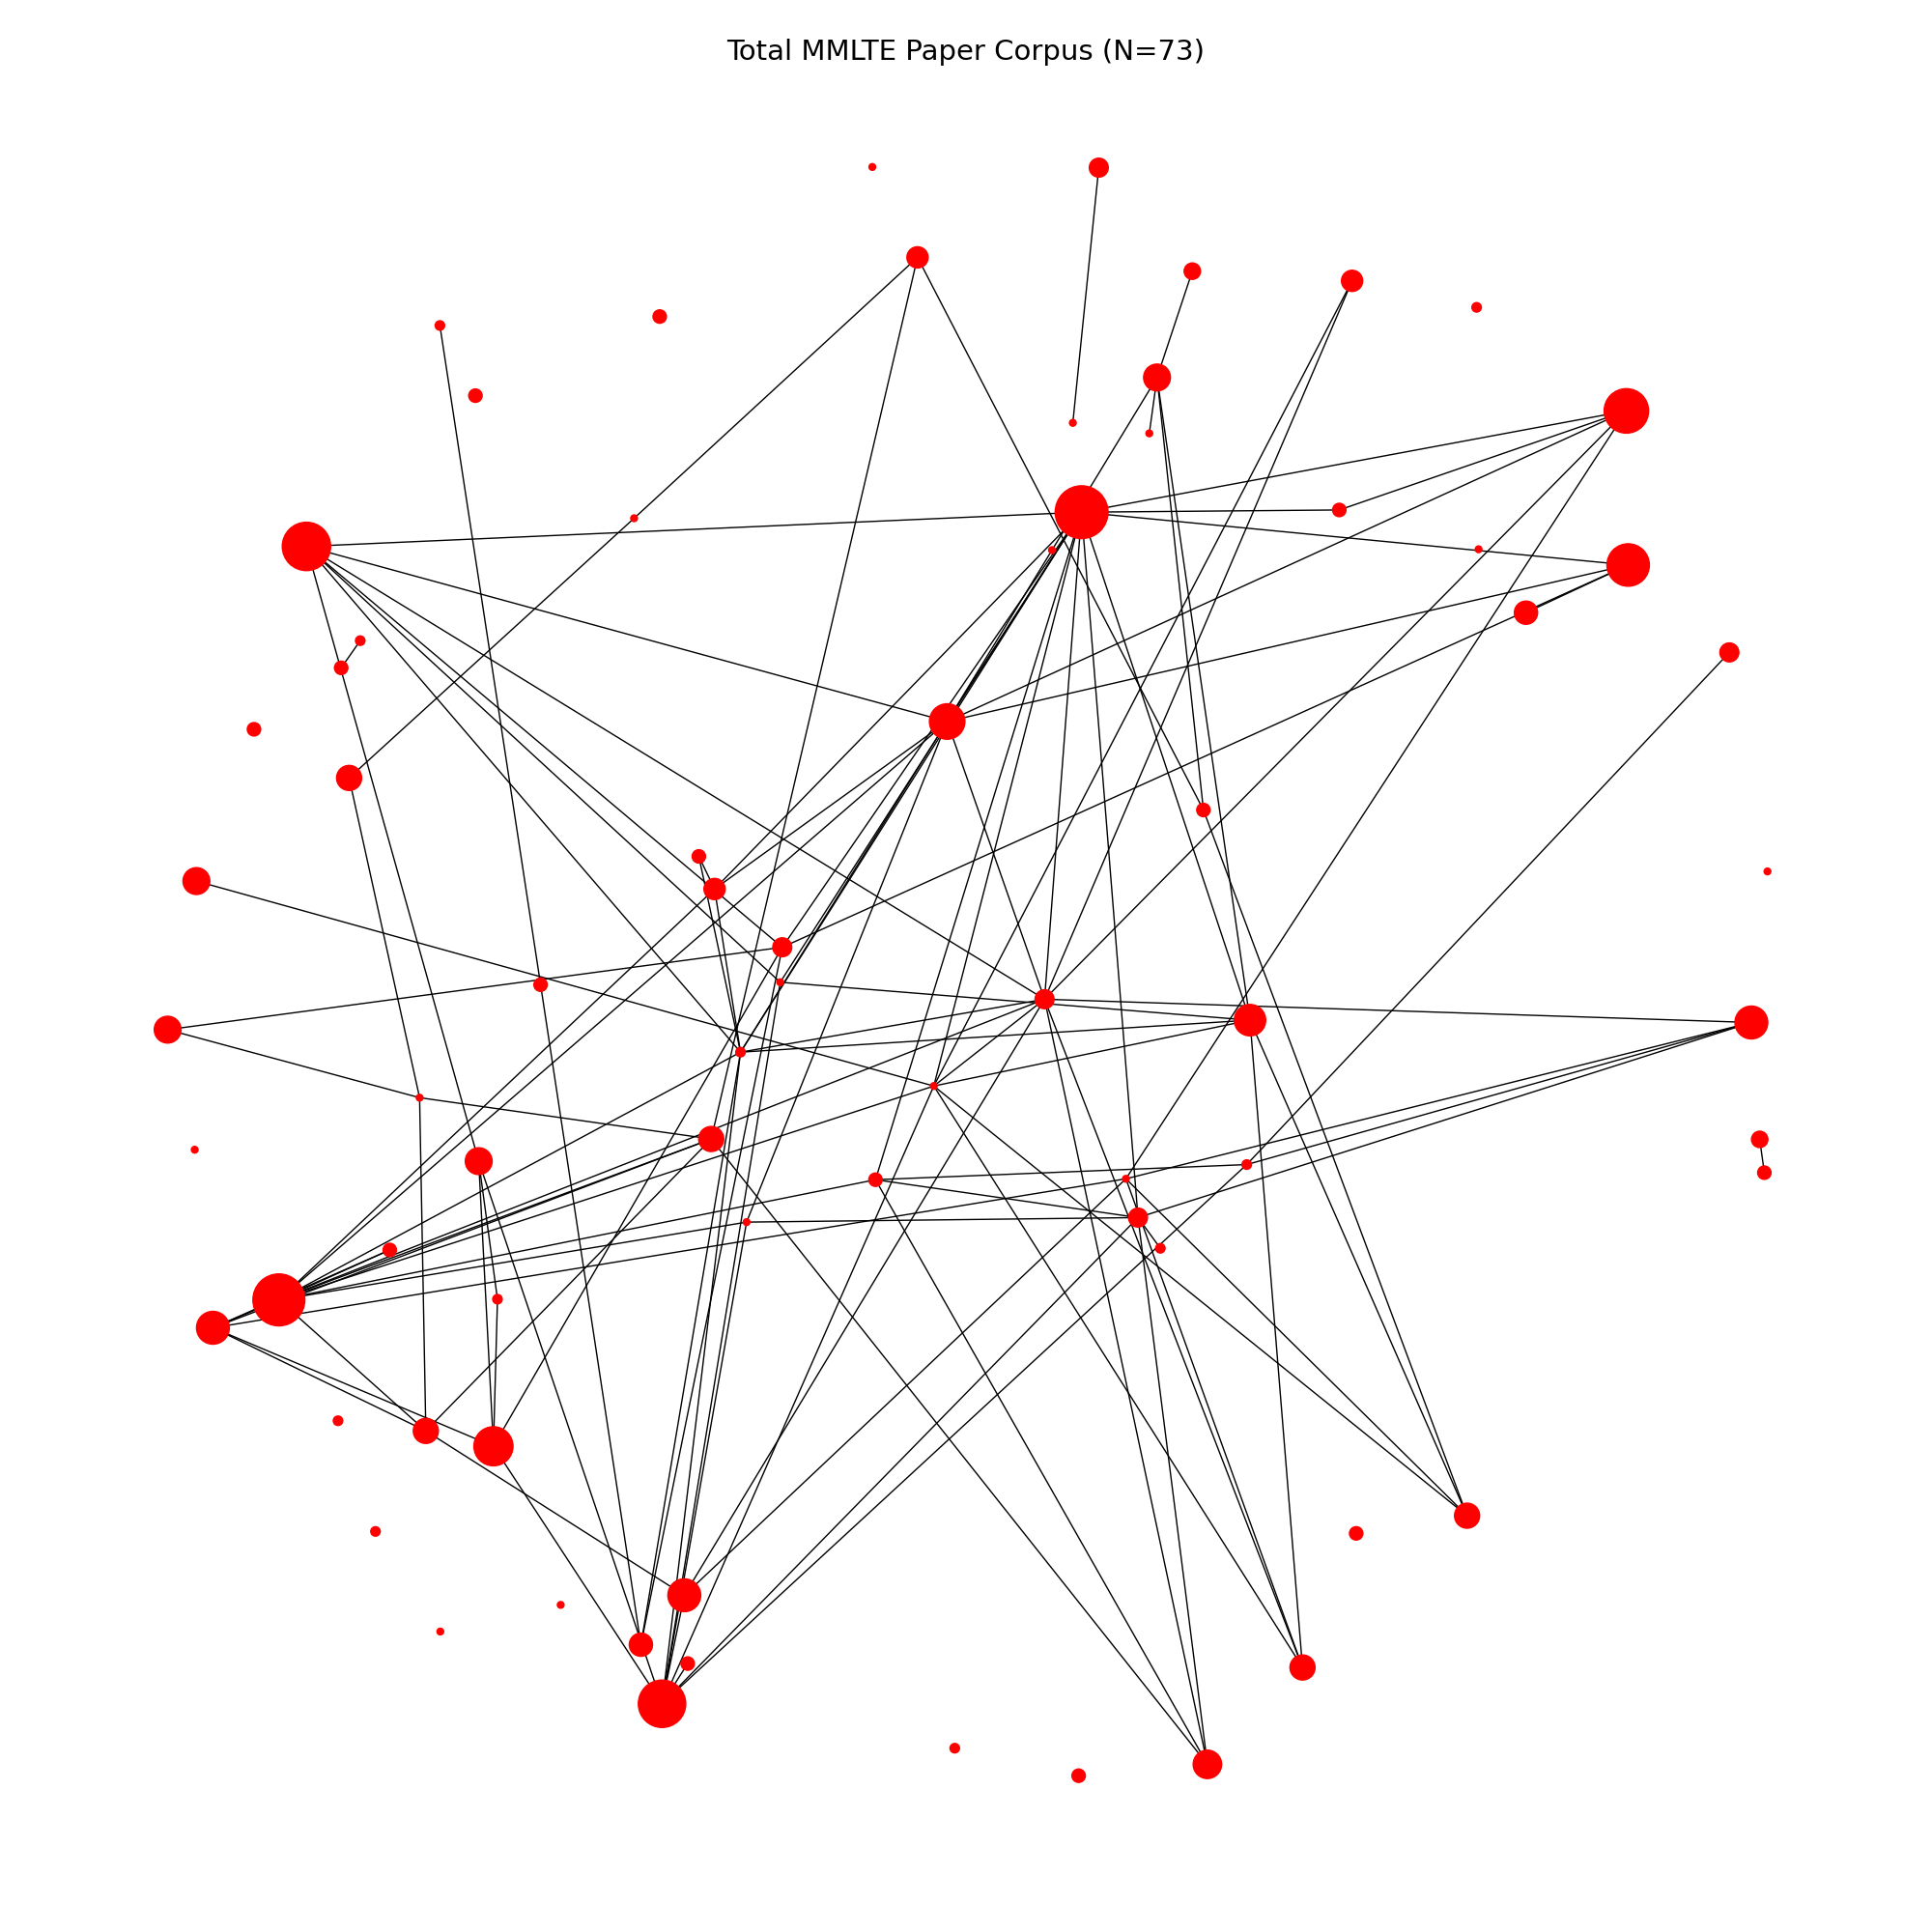
\includegraphics[width=0.5\textwidth, trim=1cm 1cm 1cm 2cm, clip]{img/community_analysis/mmlte_total_corpus_graph.png}
    \caption{Complete final corpus citation graph: }
    \label{fig:final_corpus_citation_graph}
\end{figure}

For our network approach, we started by using the citation information within our final paper corpus to create a citation graph, shown in Fig. \ref{fig:final_corpus_citation_graph}. Each node is a paper with their weight being their total citation count, rather then their citations within the corpus. This was done to verify that landmark papers were staples both within and outside our corpus.  

% Identifying Community via Louvain Algorithm
%   Louvain community discovery algorithm to generate citation communities
%   Characterized each community via their papers' extracted features
%   Computed normalized frequency for each category across the communities

\begin{figure}
    \centering
    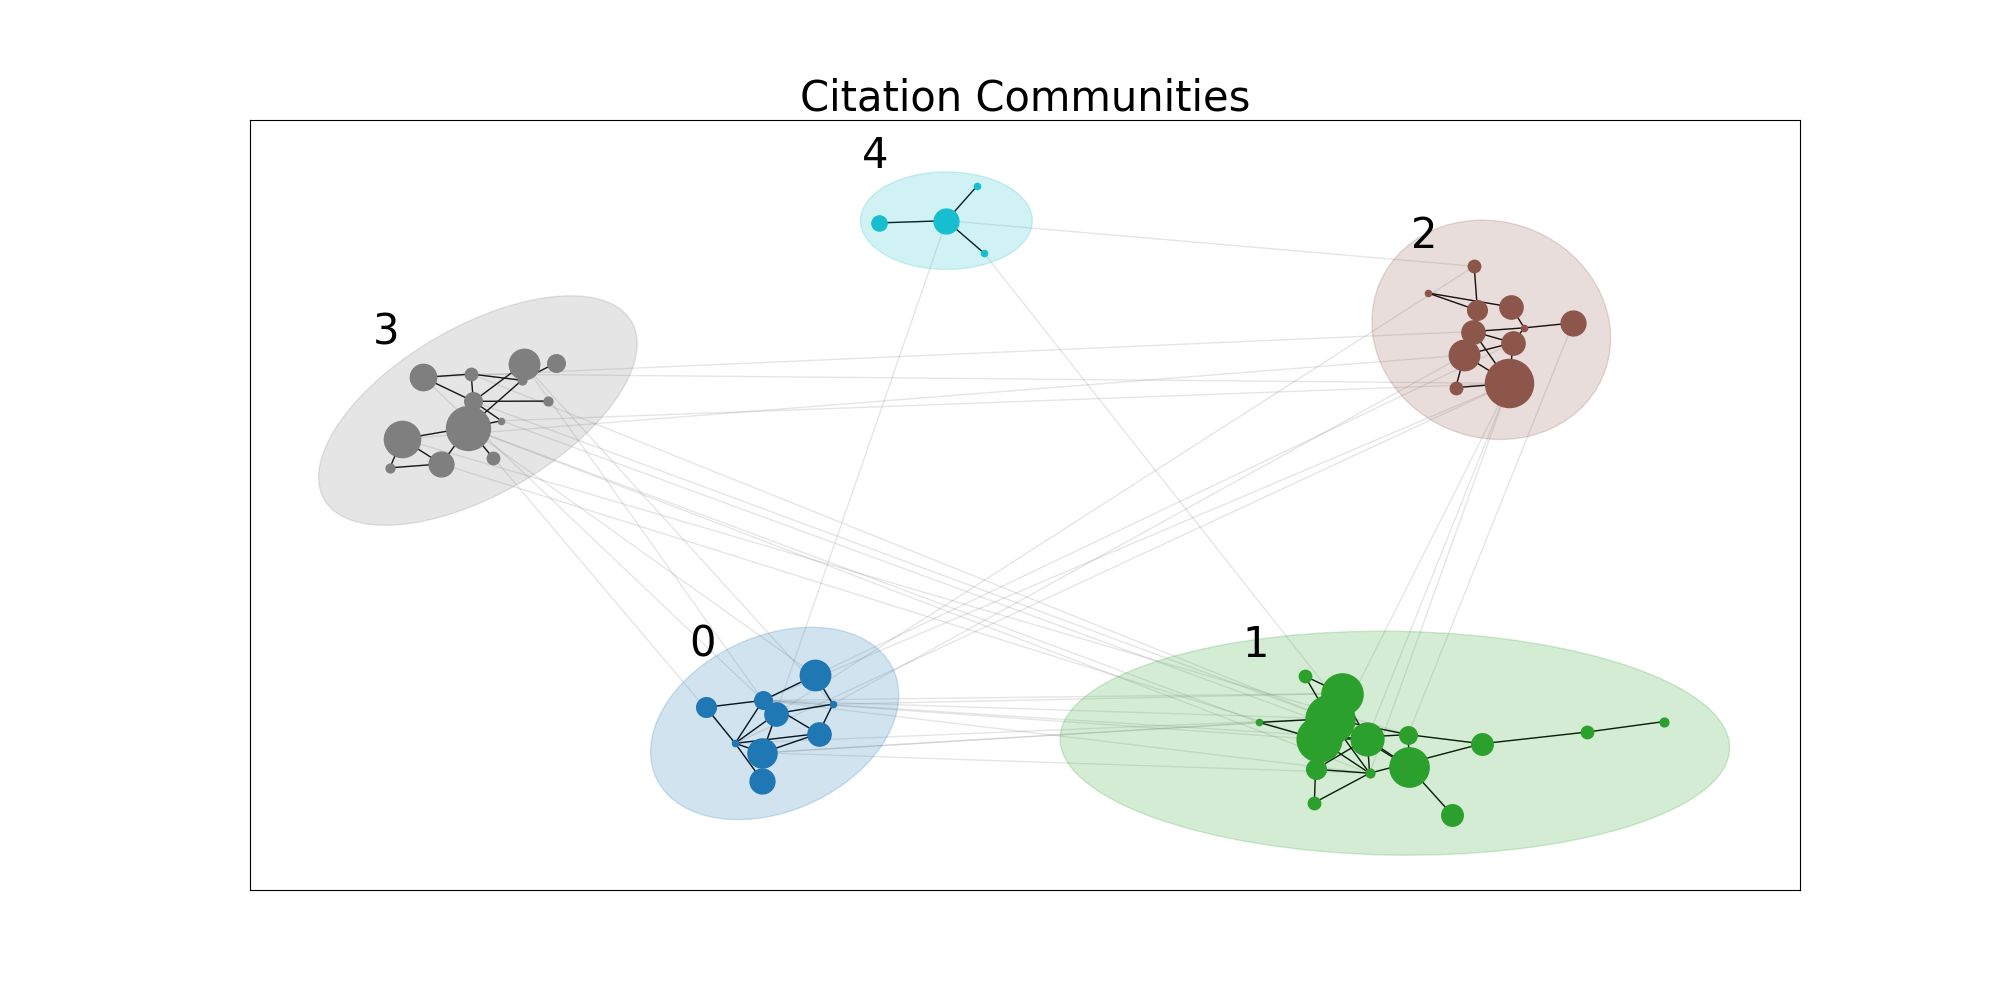
\includegraphics[width=\textwidth, trim=3cm 2cm 3cm 2cm, clip]{img/community_analysis/community_network.png}
    \caption{Identified citation communities: }
    \label{fig:citation_communities}
\end{figure}

Once with the corpus citation graph constructed, a pre-processing step was performed before using the Louvain algorithm -- Zero degree nodes within the corpus were eliminated to avoid inflating the number of identified communities. By applying the Louvain community algorithm, we obtained eight candidate communities; however, three were discarded for being two-node communities, resulting in five prominent communities. These communities are shown in Fig. \ref{fig:citation_communities}. Understanding how these communities was approached using the discrete circumscribing features through a frequency-based strategy. Across each feature category (e.g. fusion, analysis, modalities), the normalized frequency for each discrete label was computed across each community. To achieve this, each paper's discrete tags were binarized using \href{https://scikit-learn.org/stable/index.html}{Scikit-Learn's} MultiLabelBinarizer. Frequency counts of binary labels were then computed and normalized across community and category. Employing these normalized frequencies, we applied a qualitative approach supported by cosine similarity to hierarchical split communities in an inverted tree fashion, as shown in Fig. \ref{fig:qualitative_breakdown}. Beginning with all communities grouped together, a cosine similarity metric was used to split a group into subgroups by computing the similarity between intra- and inter-groups elements. The splitting processed persisted until a group contained a single community. These groups were then characterized by qualitative observing the normalized frequency differences during each split.

\begin{figure}
    \centering
    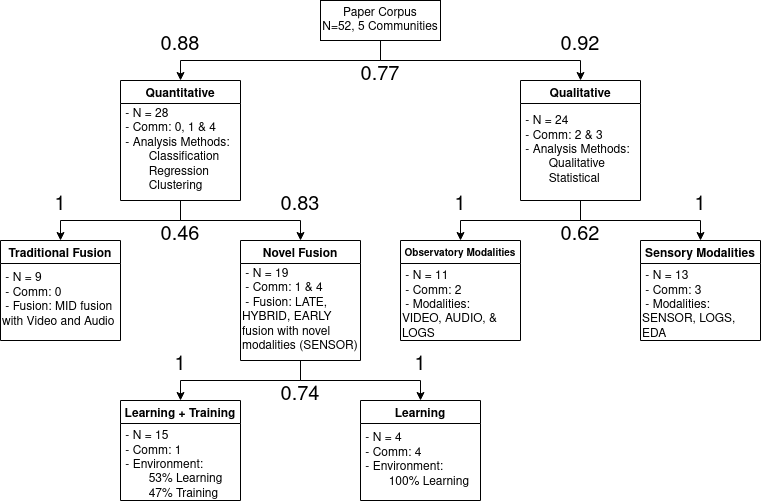
\includegraphics[width=0.8\textwidth]{img/community_analysis/Community Breakdown-Latest.drawio(1).png}
    \caption{Qualitative breakdown of citation communities using features: }
    \label{fig:qualitative_breakdown}
\end{figure}

\begin{figure}
    \begin{tabular}{|c|c|}
        \hline
        Comm. ID & Papers \\
        \hline
        0 & A \\
        1 & B \\
        2 & B \\
        3 & B \\
        4 & B \\
        None & \\
        \hline
    \end{tabular}
    \caption{Main caption for the figure}
    \label{fig:corpus_table}
\end{figure}

\section{Findings} \label{sec:findings} 
% Primary uses of multimodal analysis in MMLTE
% Discuss the need for mid-fusion versus early fusion

\subsection{Corpus Statistics}

\begin{figure}[h!]
    \centering
    \begin{subfigure}[b]{0.45\textwidth}
        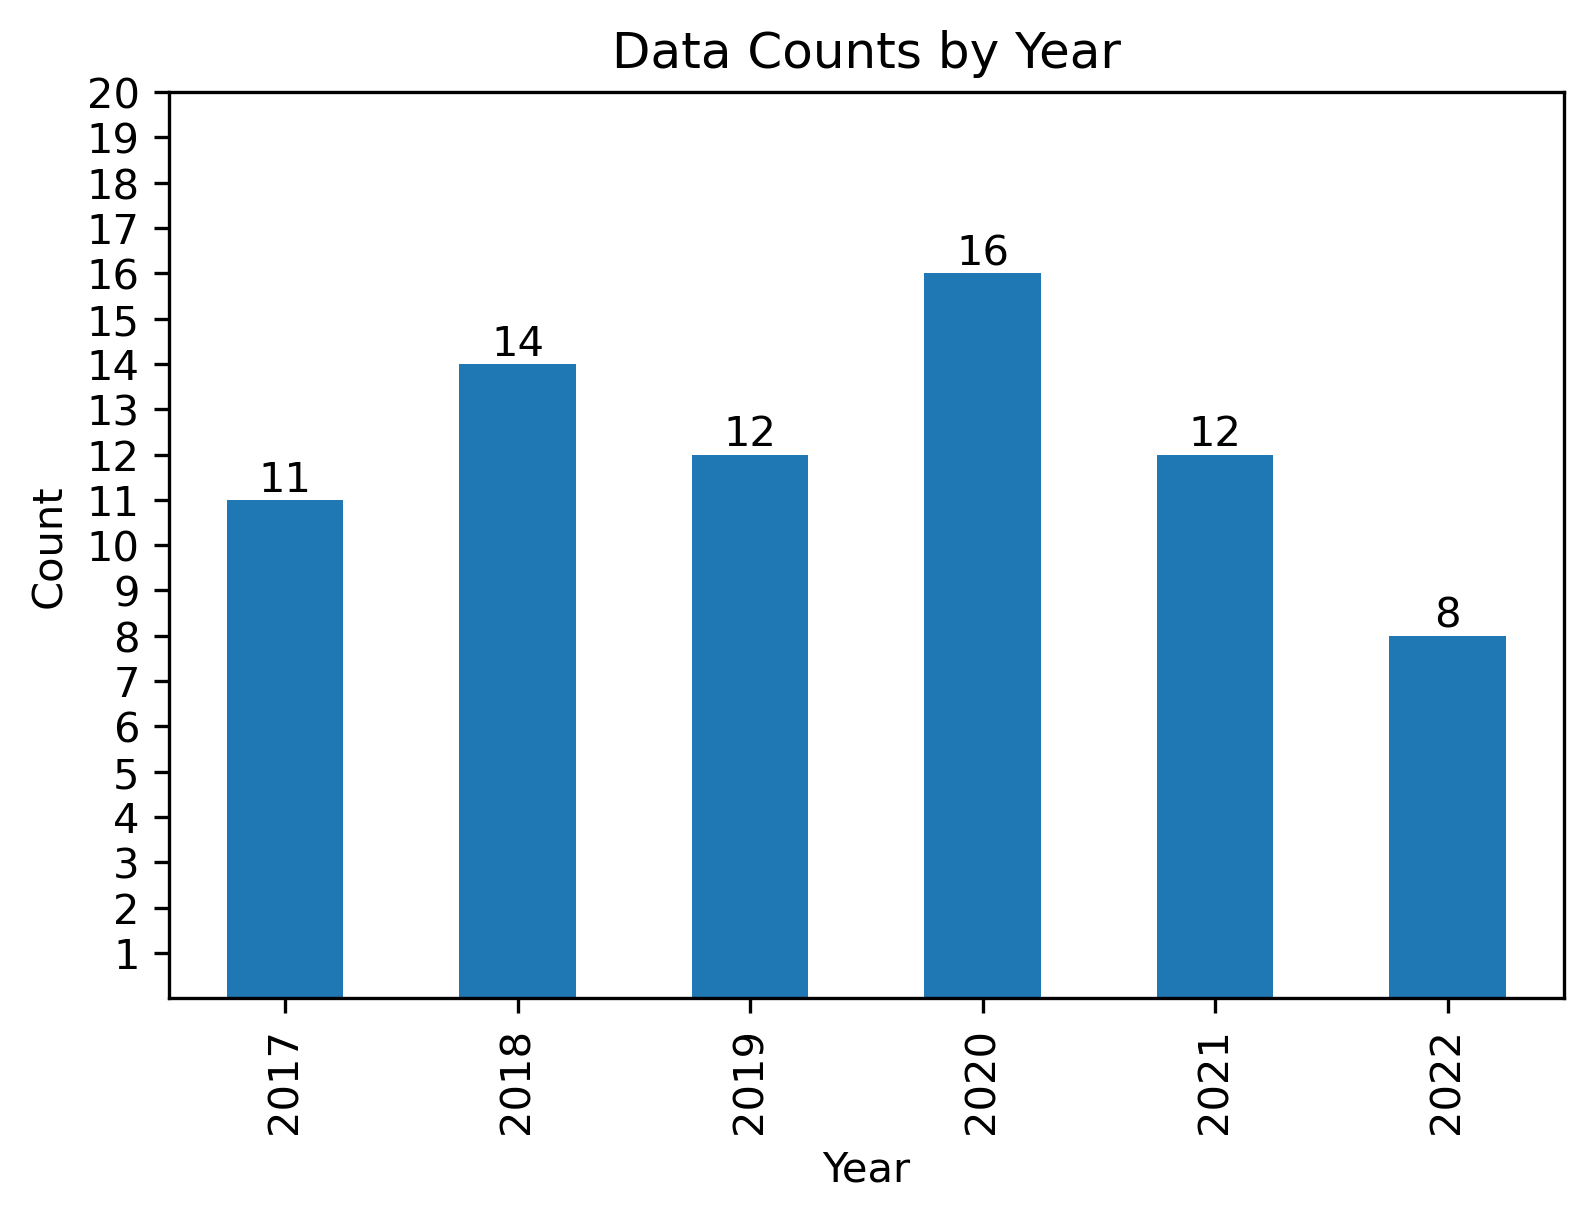
\includegraphics[width=\textwidth]{img/statistical_imgs/year.png}
        \caption{Image 1}
    \end{subfigure}
    \hfill
    \begin{subfigure}[b]{0.45\textwidth}
        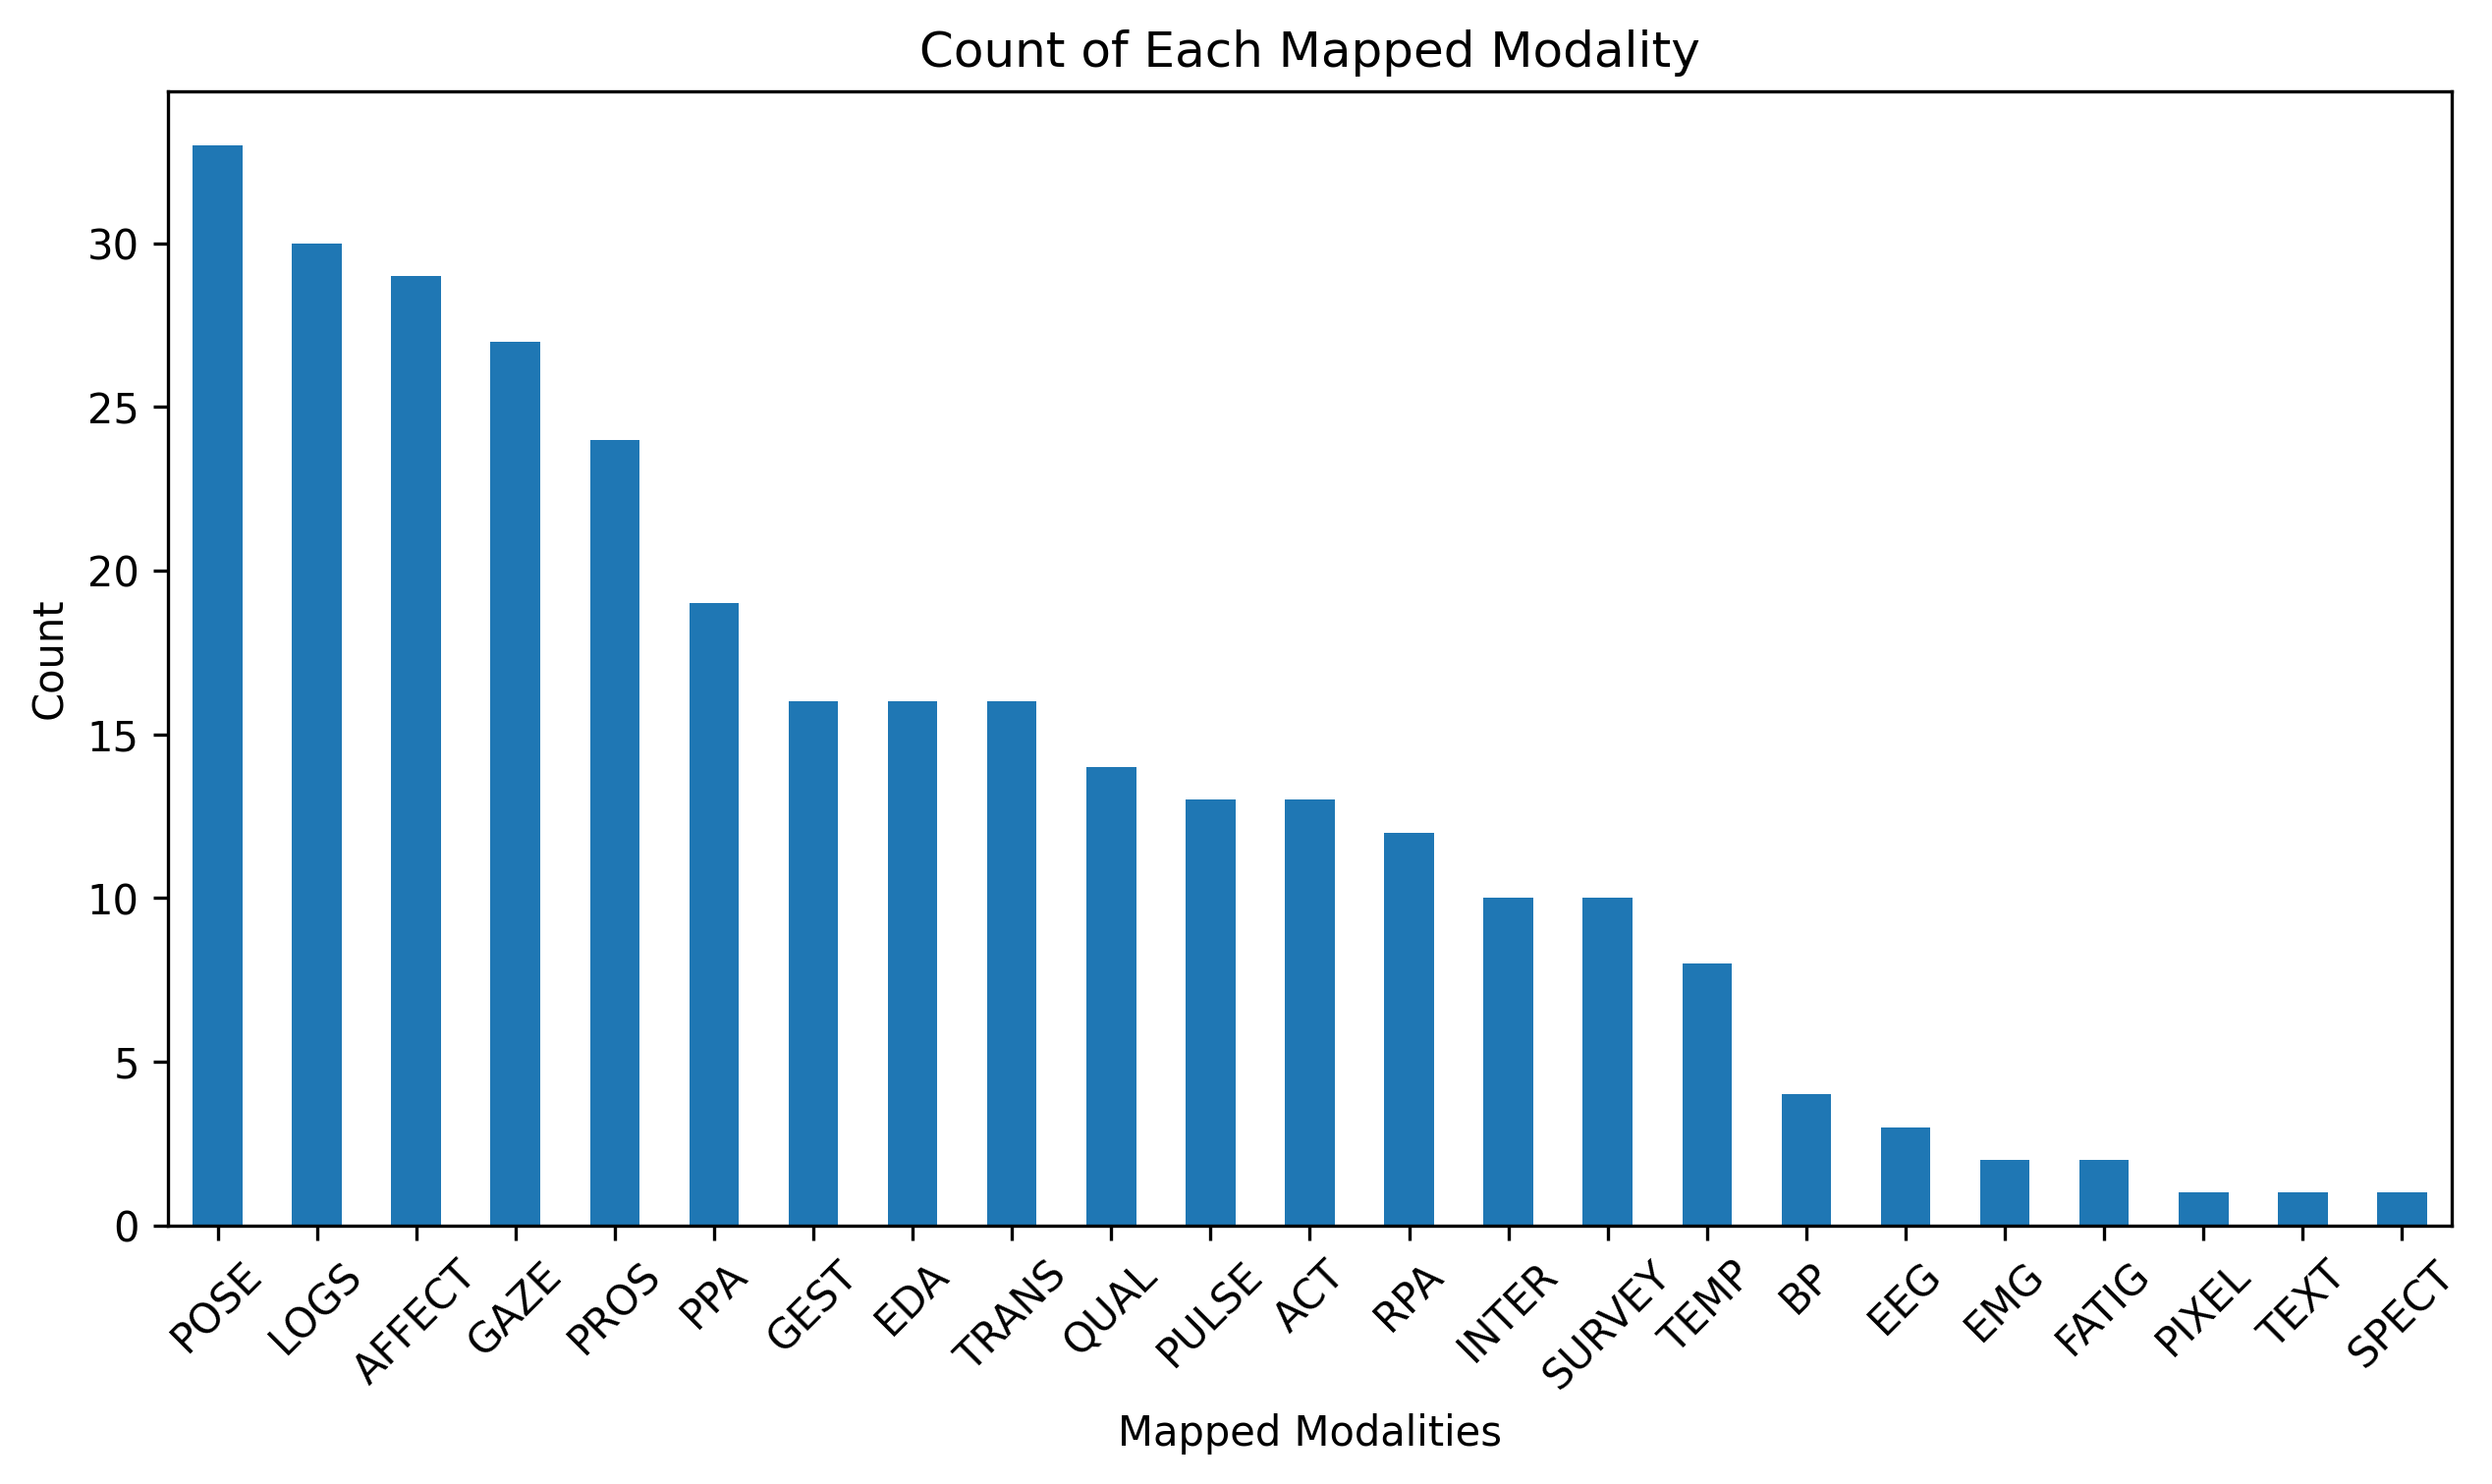
\includegraphics[width=\textwidth]{img/statistical_imgs/modalities.png}
        \caption{Image 2}
    \end{subfigure}
    \hfill
    \begin{subfigure}[b]{0.45\textwidth}
        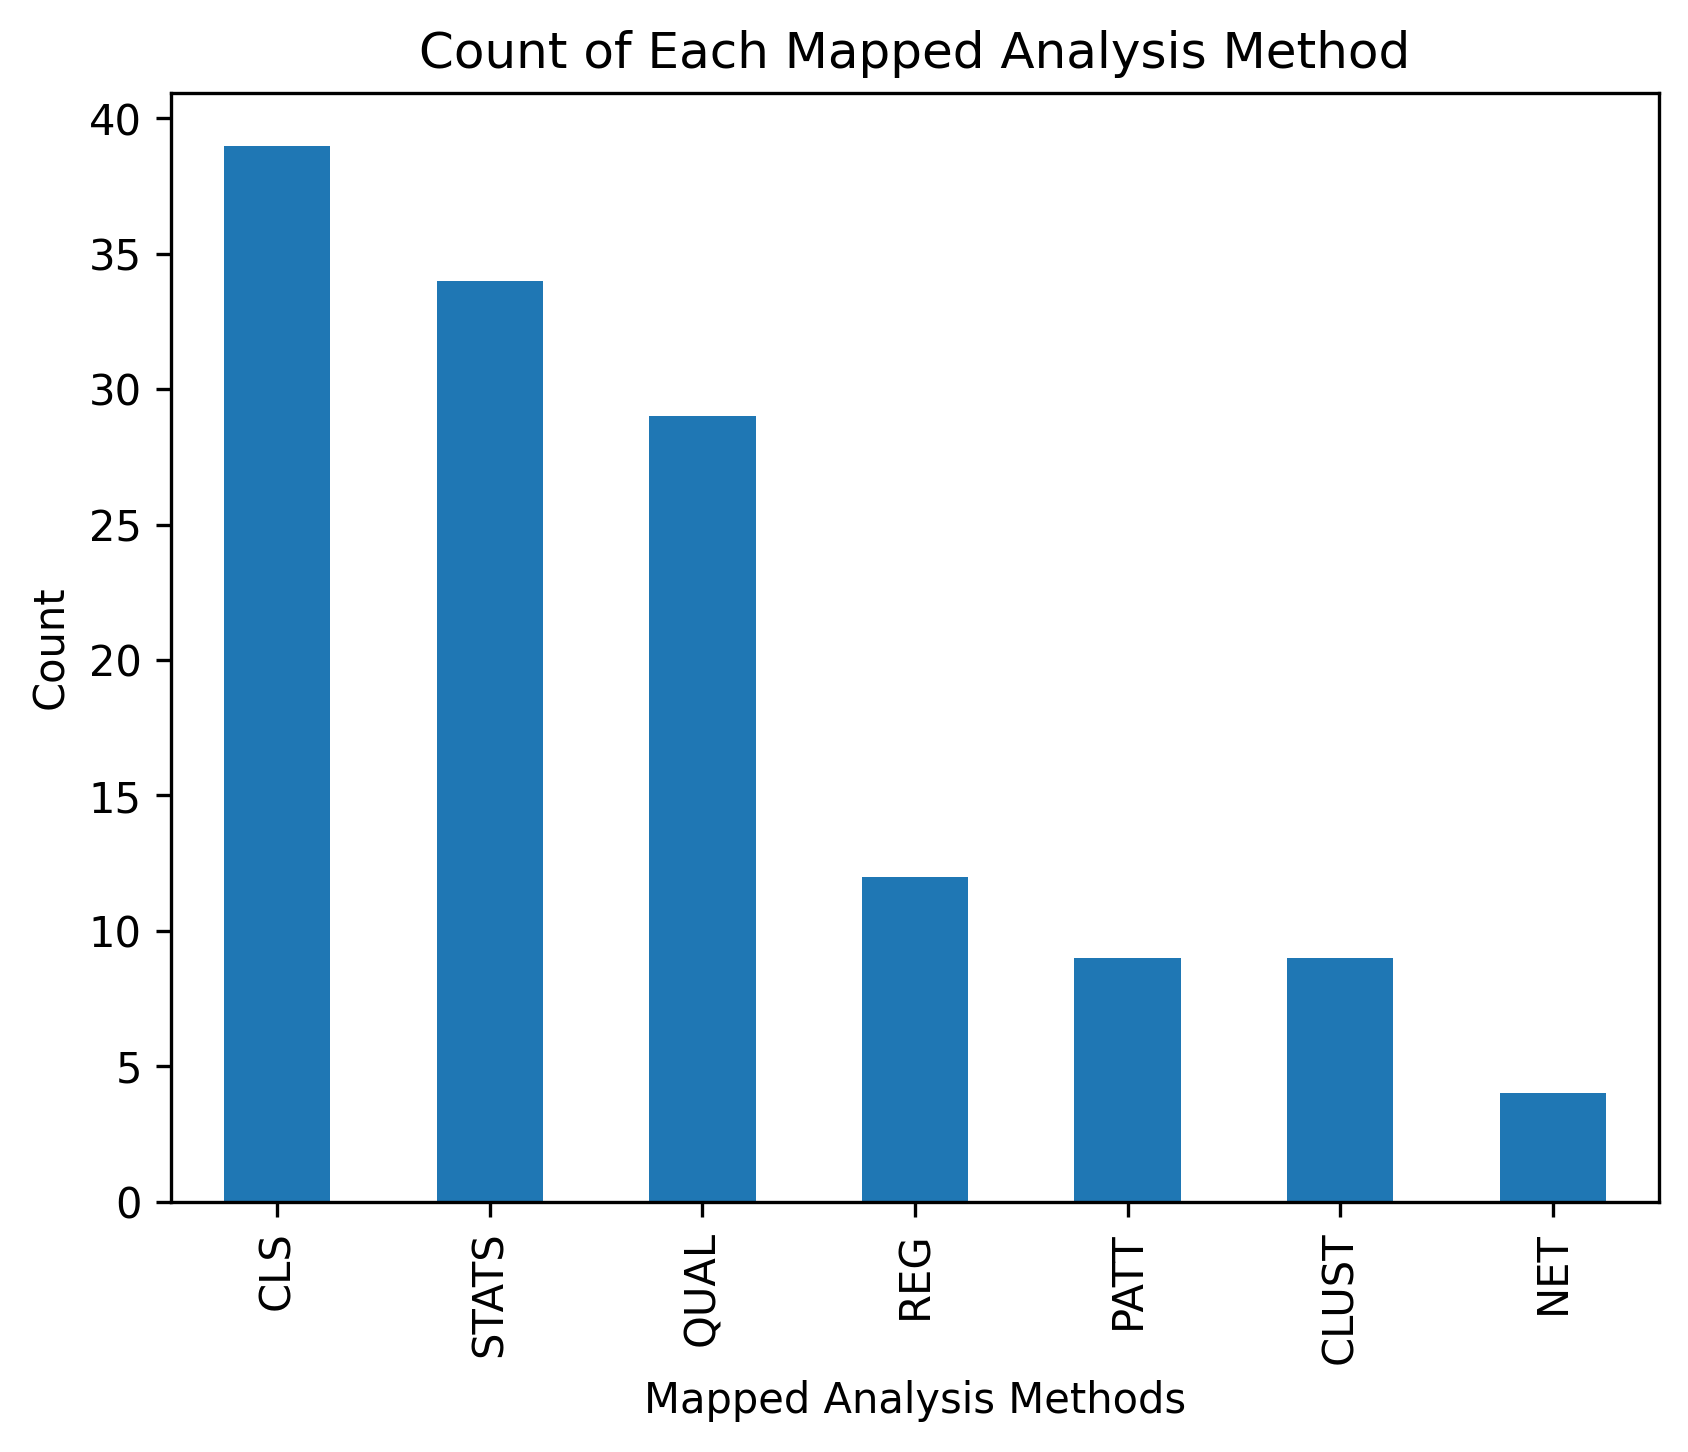
\includegraphics[width=\textwidth]{img/statistical_imgs/analysis_type.png}
        \caption{Image 3}
    \end{subfigure}
    \hfill
    \begin{subfigure}[b]{0.45\textwidth}
        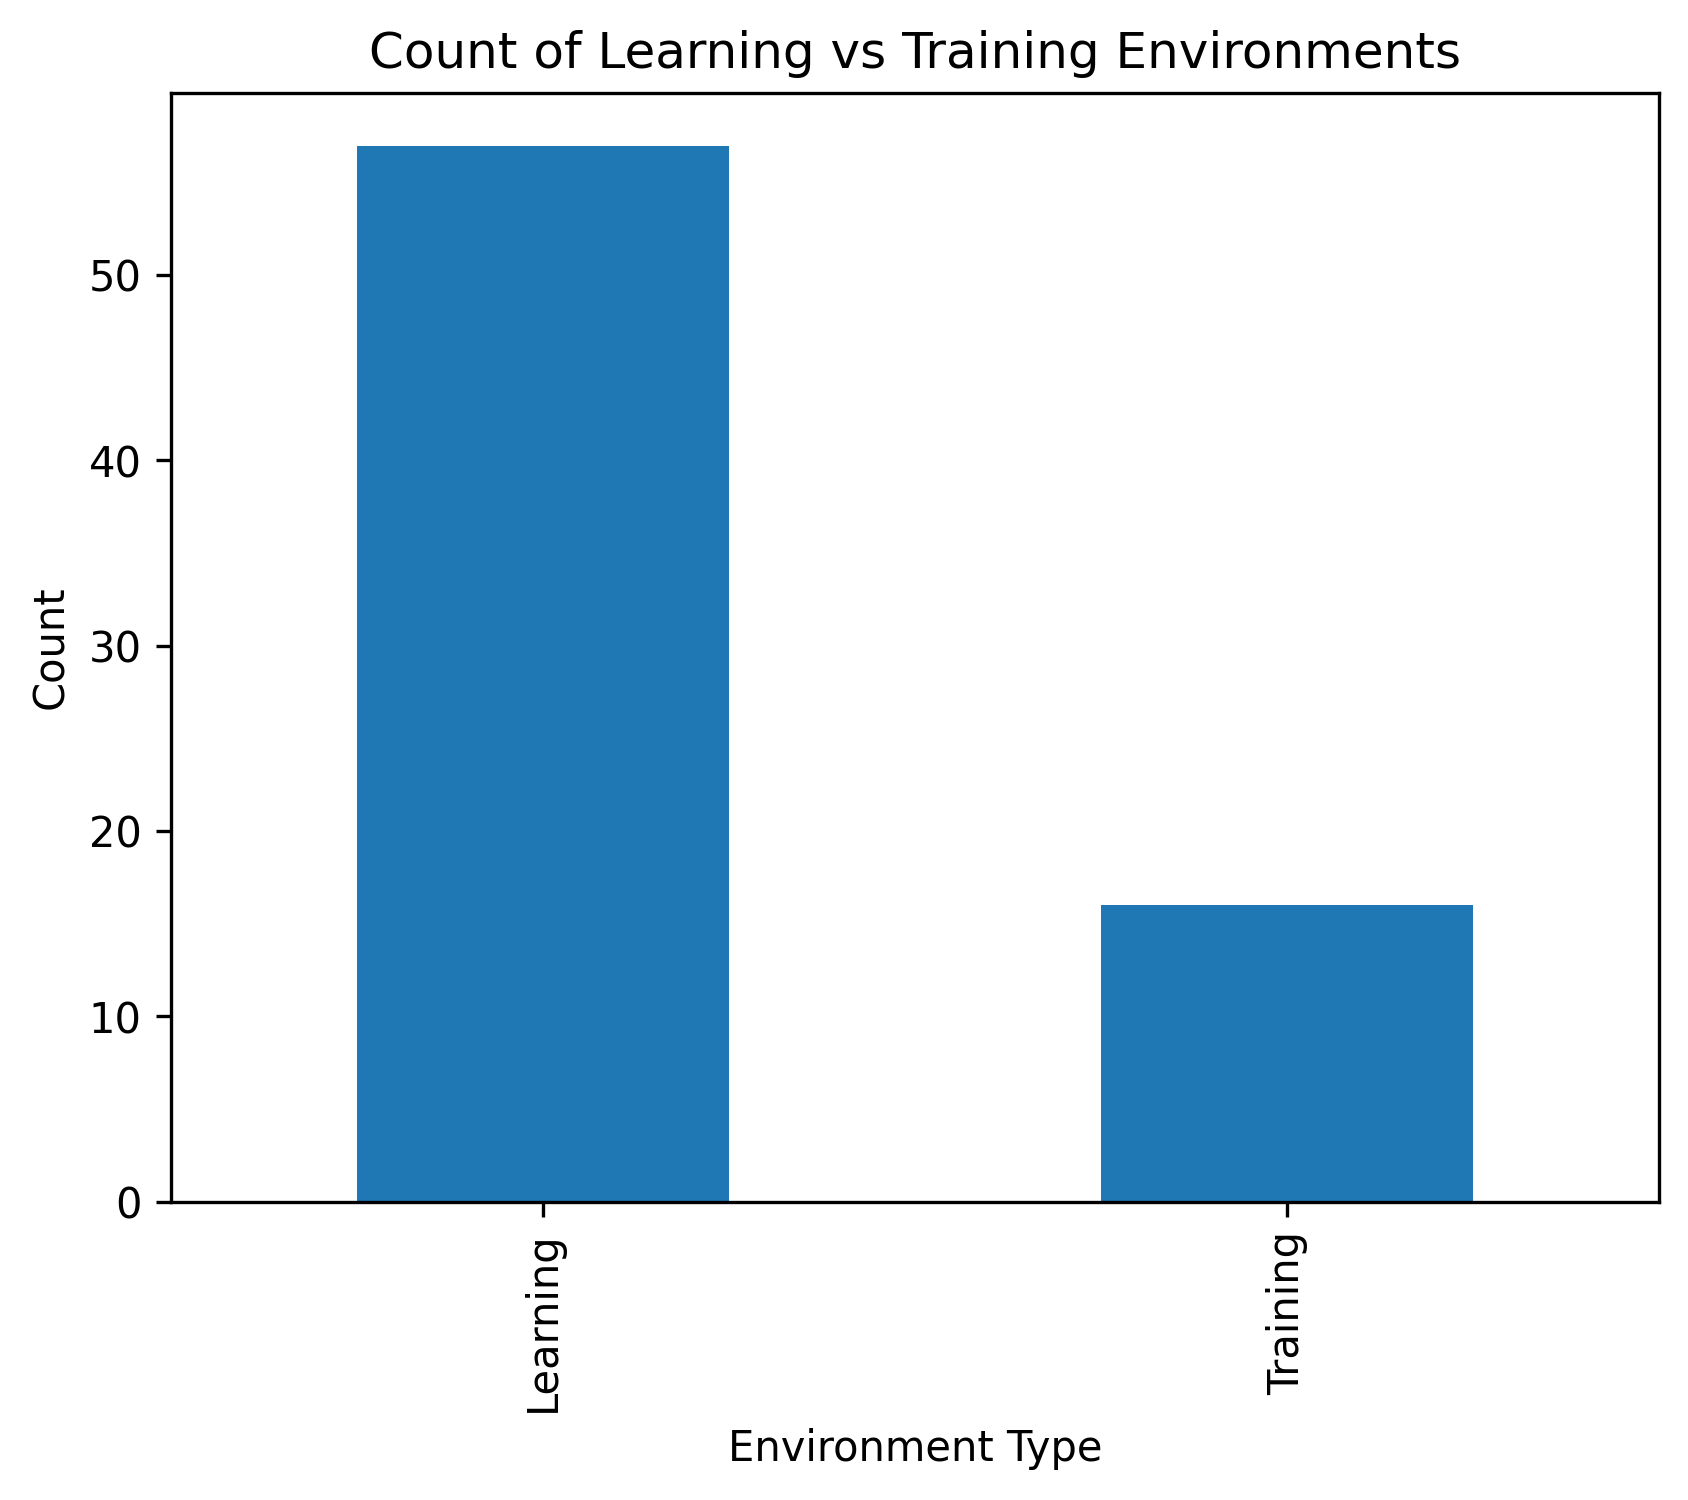
\includegraphics[width=\textwidth]{img/statistical_imgs/learning_vs_training_envs.png}
        \caption{Image 4}
    \end{subfigure}
    \\
    \begin{subfigure}[b]{0.33\textwidth}
        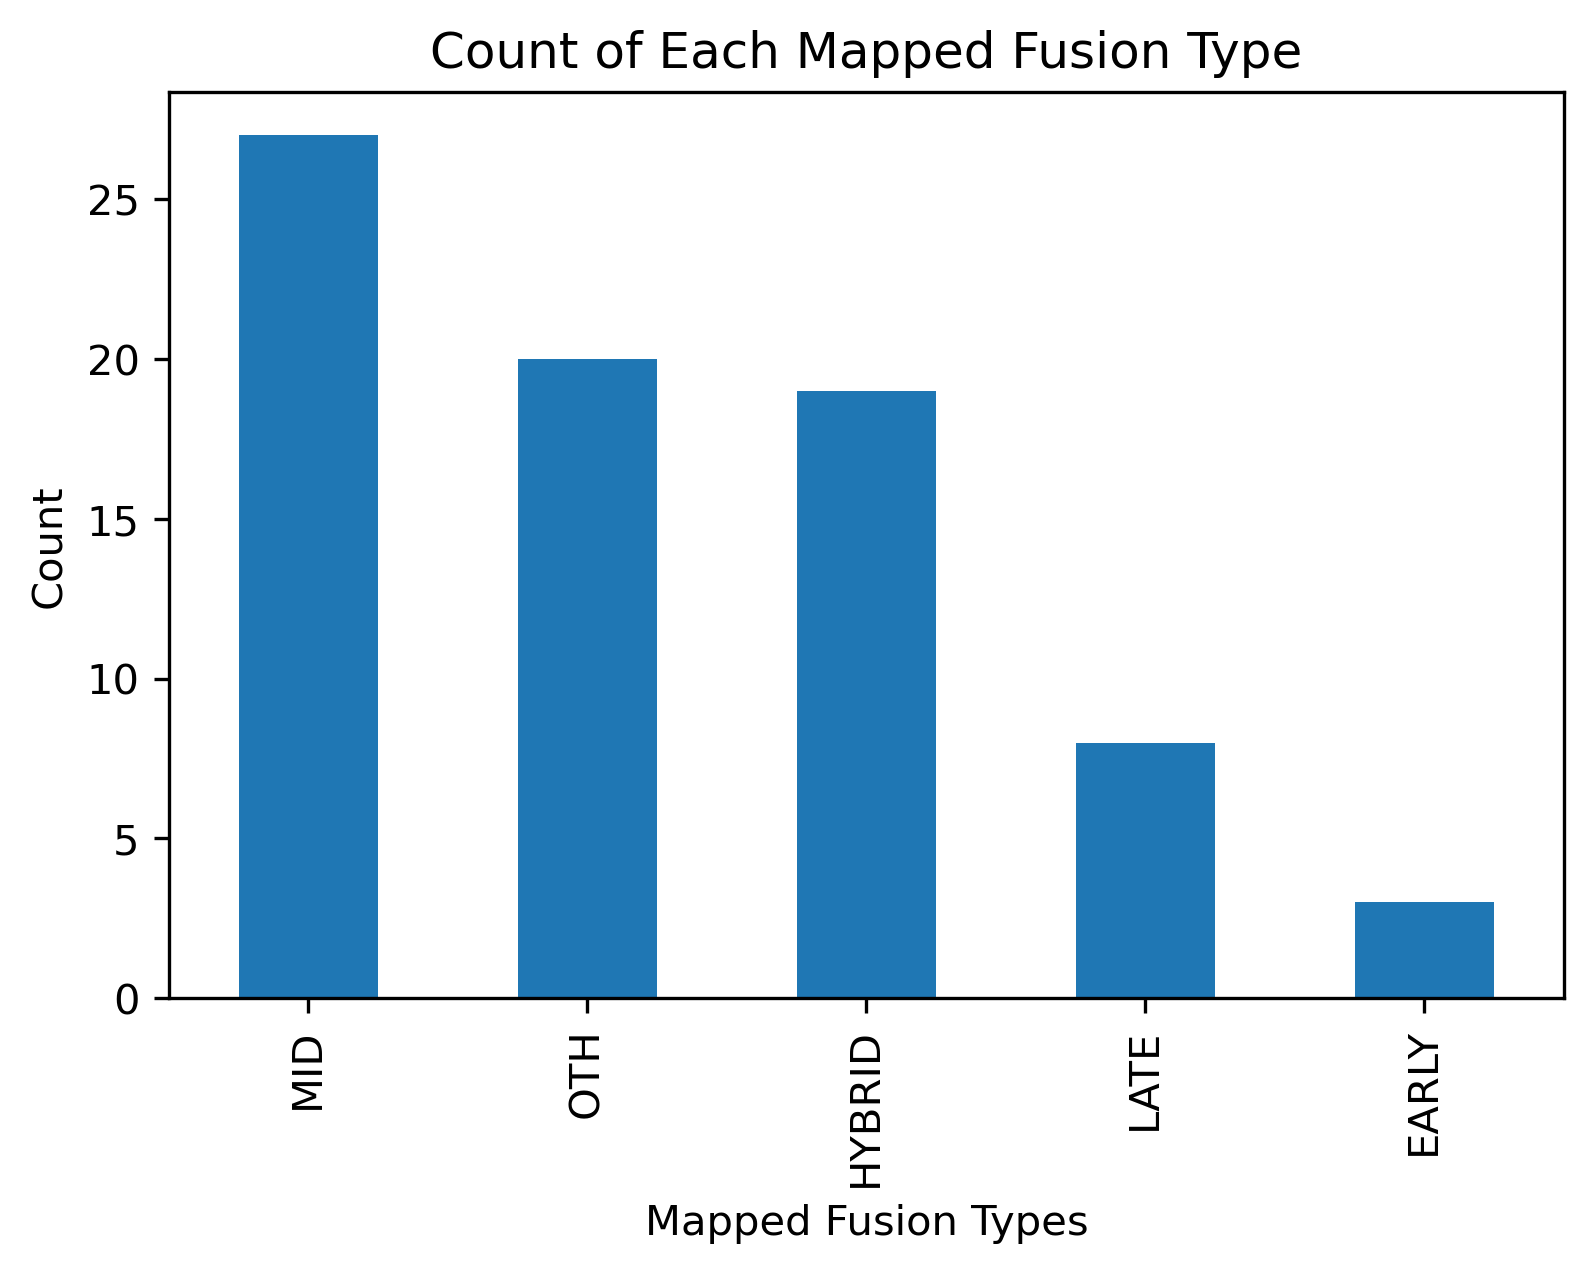
\includegraphics[width=\textwidth]{img/statistical_imgs/fusion_type with OTH.png}
        \caption{Image 5}
    \end{subfigure}
    \hfill
    \begin{subfigure}[b]{0.33\textwidth}
        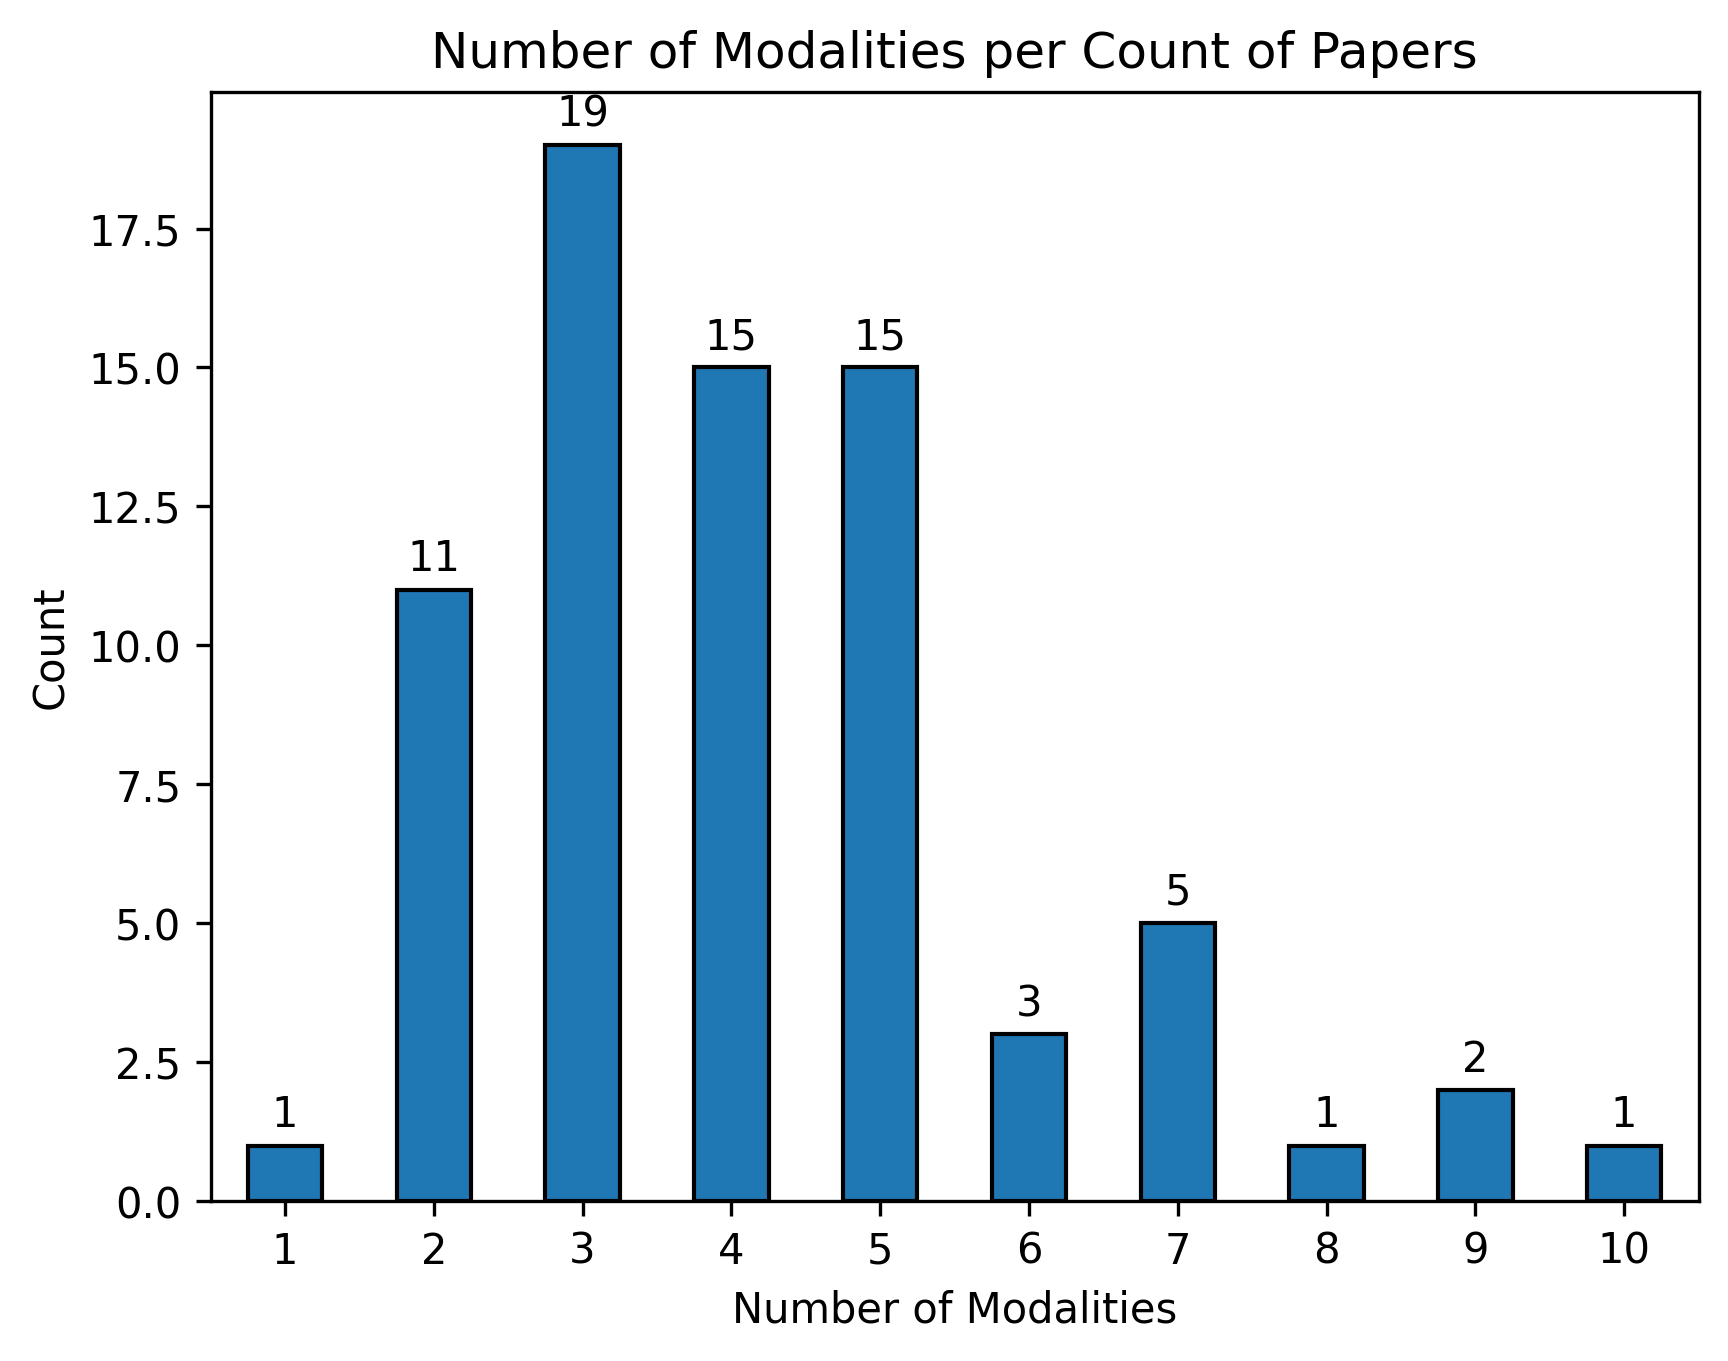
\includegraphics[width=\textwidth]{img/statistical_imgs/number of modalities per count of papers.png}
        \caption{Image 6}
    \end{subfigure}
    \hfill
    \begin{subfigure}[b]{0.33\textwidth}
        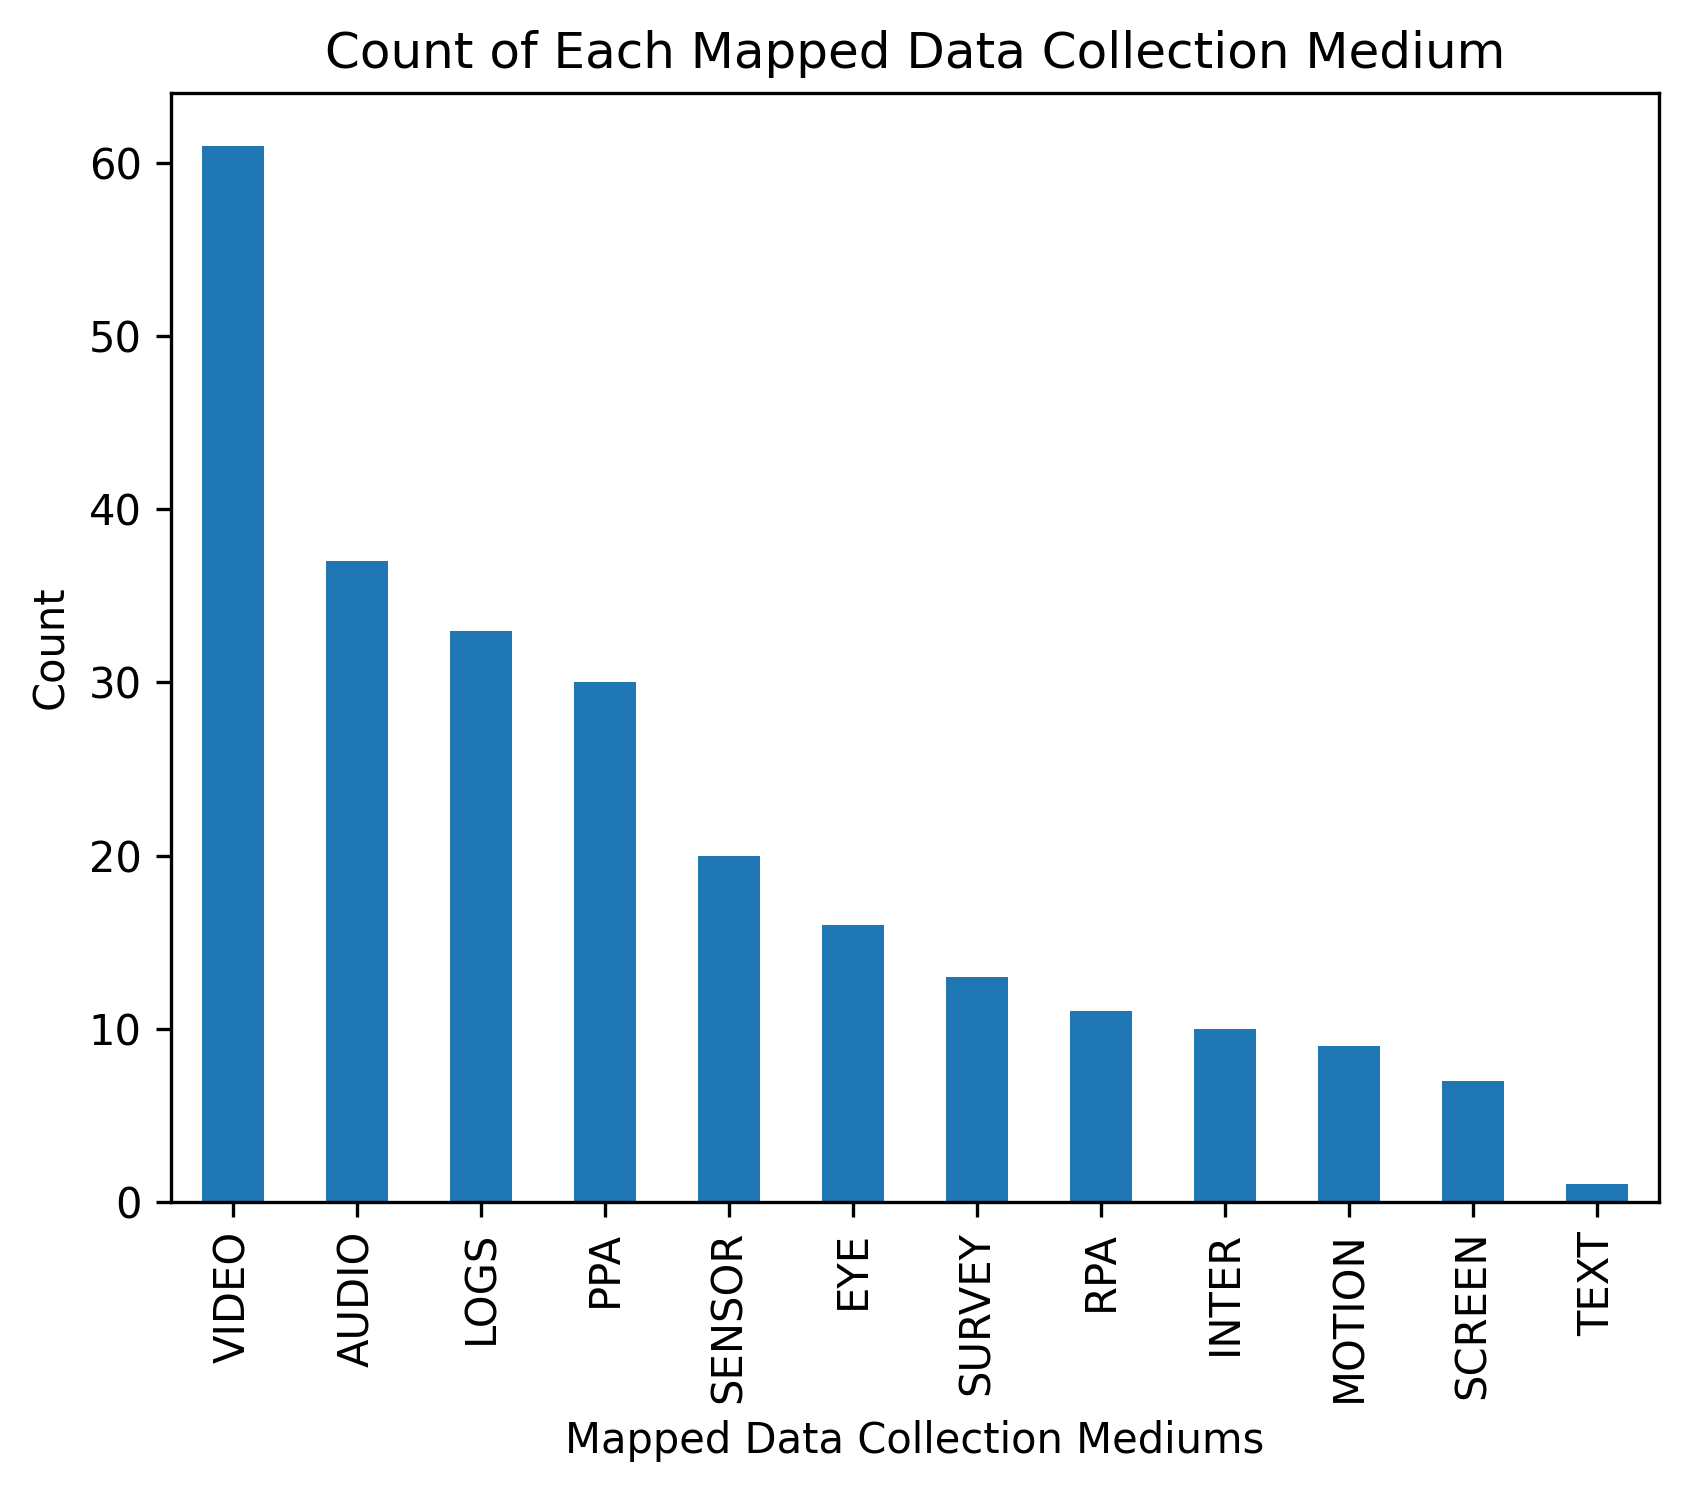
\includegraphics[width=\textwidth]{img/statistical_imgs/data_collection_mediums.png}
        \caption{Image 7}
    \end{subfigure}
    \\
    \begin{subfigure}[b]{\textwidth}
        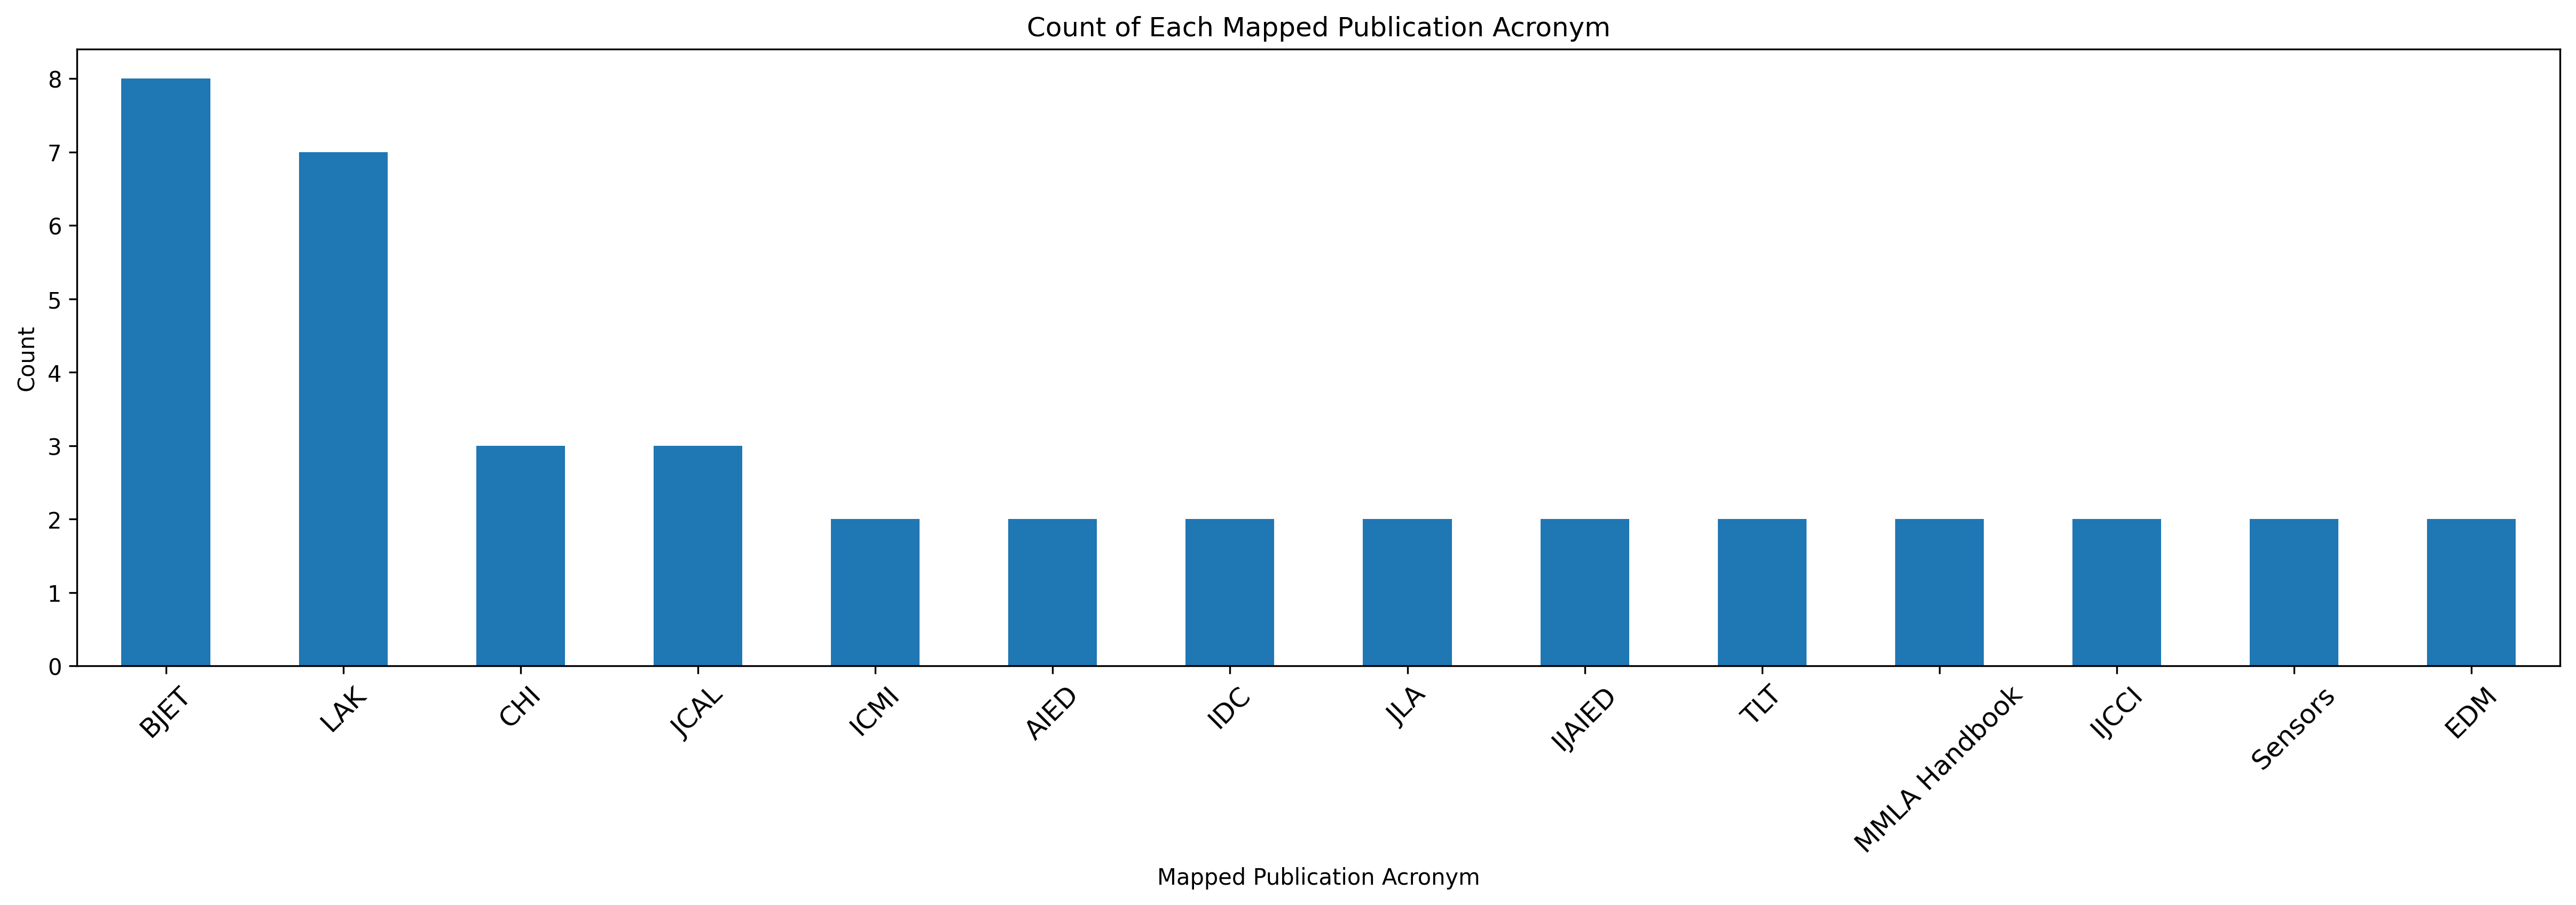
\includegraphics[width=0.8\textwidth]{img/statistical_imgs/publications_w_o_others.png}
        \caption{Large Image}
    \end{subfigure}
    \caption{Composite figure with 7 small images and 1 large image}
\end{figure}

% Papers over time, David
% Learning v. training envs, David
% Fusion type/bar chart, David
% Analysis type/bar chart, David
% Modalities bar charts, David
% Mediums bar charts, David
% Publications bar chart, David
% Number of papers per number of modalities, David

\subsection{Citation Community} % Eduardo
%########################################################################################
% Eduardo's Email Regarding communities, for reference

% Hello MMLTE Team,

% Apologies for the delay on the community analysis, surprisingly difficult to do anything with KB internet.

% I was able to perform the community analysis and it provided an interesting perspective on the MMLTE body of literature. I have attach some preliminary figures that I have created to help understand the results. I also provide a zip file with more information. 

% Let me first breakdown the approach and please let me know if you find any faults, concerns, or invalid practices.

% # Preprocessing
% For the community detection, I remove all 0 degree Nodes (as these wouldn't be part of any community and combine these into a community didn't seem appropriate due to their lack of relationship). This removal reduced the corpus from 73 to 58. After detecting the communities, I also removed all communities smaller than 3 nodes, as I noticed that communities of 2 were highly homogeneous in their categorical attributes (modalities, fusion, and analysis). There were like a continuation of prior work but didn't resemble a trend or an actual community of research in MMLTE. This removal step reduced the corpus from 58 to 52.

% # Analysis
% After the preprocessing step, the communities were detected by the louvian community detection algorithm from this package, resulting in 5 communities of size greater than 3 from the 52 paper corpus. The following sizes of the each of the communities are the following:

% 0: N=9
% 1: N=15
% 2: N=11
% 3: N=13
% 4: N=4

% It was difficult to understand how these communities were different or similar at first, but I thought that I could use the discretize attributes (modalities, fusion, and analysis) to explore patterns and differences between the communities. For each community, I computed the normalized (sum/total) frequency counts of each category. Then I created a (dense) heatmap visualization across the modalities, fusion types, analysis methods and environment types for all the communities. I can create a separate figure with each column for clarity if needed, but the collective figure is more helpful for recognizing the differences and similarities between the communities.

% With the comprehensive normalized frequency figure, I was able to create a tree that separates and characterized the communities. I noticed that communities are split by their methodology (QUAN vs QUAL). The QUAN branch is further split by the fusion and modality types. For the QUAL branch, the split is from the types of modalities used observatory (e.g. VIDEO, AUDIO, and LOGS) vs sensory (e.g. SENSOR, EYE, and LOGS). A figure displaying this tree is also attach to this email to further clarify.

% Any thoughts or feedback would be greatly appreciated!

% Best,
% Eduardo Davalos
% ########################################################################################

% Qualitative description of the community based on their relative frequency along with cosine similarity
%   Inverted Tree breakdown

% Summary of Network Analysis
%   QUAL vs QUANT
%   QUANT has major splits between traditional MID and experimental modalities & fusion types
%   QUAL split between observatory and sensory modalities

\section{Discussion} \label{sec:discussion}
% Recap what we have done and findings

% Comprehensive review of research methods applied to multimodal learning and training environments
% Qualitative analysis of current body of literature based on environments, authors, year, modality, medium, fusion, analysis type, publication
% Need for mid fusion
% A novel citation graph method for corpus reduction
% Categorization and description of MMLA literature via citation communities
% Also discuss implications, limitations, and future research directions with MMLA

\subsection{Implications}
% Findings:
% BJET and LAK most popular journal/conference for applied MMLA and quantitative analysis
% Learning more popular than training currently
% Video, audio, logs, ppa most popular mediums
% Pose, logs, affect, gaze, and prosodic speech appear to be the most popular modalities.
% Most multimodal work considers 2-5 modalities per paper
% Classification, stats, qual most popular analysis methods
% Mid fusion and hybrid fusion most popular
% 5 Communities

% Not necessary to do tons of modalitites, but focus on a few that are the most informative
% Should consider data fusion to inform environment, particularly mid fusion by fusing observable, derived features
% Use communities analyis to inform your own multimodal research 

\subsection{Limitations}
The major limitations of this work involve the use of Google Scholar to conduct the literature search and the use of a citation graph for programmatic corpus reduction. Both are discussed in the following paragraphs.

\subsubsection{Google Scholar.} While Google Scholar is widely used by researchers across both academia and industry, it poses a challenge for reproducibility. Like Google Search, Google Scholar is a non-deterministic, proprietary search algorithm. Factors such as the individual user conducting the search, the user's geolocation, the date the search was conducted, and the user's search history may all affect how Google Scholar collates search results. Google may also perform A/B testing in live environments to determine which version of its algorithm users deem more effective. The algorithm is also (presumably) continually evolving, and users are unable to know exactly which version of the algorithm is used to conduct a particular search. As such, there is little expectation that our initial corpus will be able to be reconstructed \textit{in its exact form} without at least some degree of variability.

The authors are confident the degree of variability from different Google Scholar searches does not prohibit the \textit{overall} reproducibility of the initial corpus. While SerpAPI's web scrape method is proprietary, the creators address several of our concerns in their documentation\footnote{https://serpapi.com/}. The API's search does not use information from any individual user's Google account when conducting the web scrape, as no Google account is attached to the SerpAPI account, API key, or API calls themselves. Instead, calls are made via proxy and random headers, as illustrated in Figure \ref{fig:serpAPI}. When trying to reproduce the API's results via manual search, SerpAPI recommends using the URL in the API's JSON results in ``incognito mode". 

\begin{figure}
    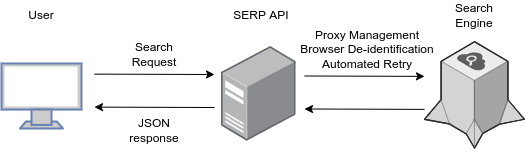
\includegraphics[width=\textwidth]{img/SERP_API_diagram.drawio.png}
    \caption{Searching Google Scholar via SerpAPI.}
    \label{fig:serpAPI}
\end{figure}

Additionally, we reached out to SerpAPI directly and asked, ``Does SerpAPI attach personal or identifying information when making request?", to which SerpAPI responded, ``No, we don't add any personal information." SerpAPI also stated, ``...others can reproduce your results by using Google Scholar website, if they use the same search criteria...", but we believe this to be an overstatement given Google's lack of transparency with regard to exactly which algorithm is being used in any single search. While we cannot guarantee perfect reproducibility due to the aforementioned issues, we can state with a reasonable degree of confidence that our own individual search biases did not influence the initial search results (outside of the choosing of the search terms) due to how SerpAPI handles API calls to Google Scholar. For reference, this review's literature search was conducted by an author of this paper in Nashville, TN, USA on October 22, 2022.

\subsubsection{Citation graph pruning.} 

As discussed in Section \ref{subsec:study_selection}, we initially pruned our corpus using quantitative means via the use of a citation graph. In doing this, it is possible we excluded relevant works from our corpus based on them only having cited or been cited by a minimal number of other works in our corpus. This literature review is a survey of the prominent methods, practices, and approaches researchers are applying to multimodal learning and training environments. As such, the authors agreed that if a work did not utilize a large degree of previous research (i.e. cite several other works in the corpus) or serve as a base from which a large degree of other researchers have built upon (i.e. be cited by several other works in the corpus), then that work was likely outside the scope of our review. Considering our corpus was still largely comprised (over 50\%) of works later deemed to be outside the scope of this review after graph-based pruning, the authors are confident that few papers directly pertaining to multimodal learning and training environments were discarded as a result of graph-based pruning.

\subsection{Other Limitations}.
% Limitation for papers not peer reviewed, but this is okay because all papers accepted somewhere and therefore refereed to some degree. 

% Search term limitation add
%   we only searched "multimodal," so MMLA research done without using this word may not be included in our initial search

% ChatGPT not included

\subsubsection{Future Research Directions} 
% Additional modalities
% Text with LLMs (search ended a month prior to ChatGPT release)
% Textless NLP 
% Domain-specific directions
% Infrastructure
% ChimeraPy
% Further automating corpus reduction process

\section*{Conflict of Interest Statement}

\section*{Author Contributions}

\section*{Funding}
% All grants involved

\section*{Acknowledgments}

%%
%% The next two lines define the bibliography style to be used, and
%% the bibliography file.
\bibliographystyle{ACM-Reference-Format}
\bibliography{references, zotero_references, corpus_papers}

%%
%% If your work has an appendix, this is the place to put it.
% \appendix

\end{document}
\endinput
%%
%% End of file `sample-manuscript.tex'.
